\documentclass{report}

%%%%%%%%%%%%%%%%%%%%%%%%%%%%%%%%%
% PACKAGE IMPORTS
%%%%%%%%%%%%%%%%%%%%%%%%%%%%%%%%%


\usepackage[tmargin=1cm,rmargin=1cm,lmargin=1cm,margin=0.85in,bmargin=2cm,footskip=.2in]{geometry}
\usepackage{amsmath,amsfonts,amsthm,amssymb,mathtools}
\usepackage[varbb]{newpxmath}
\usepackage{xfrac}
\usepackage[makeroom]{cancel}
\usepackage{mathtools}
\usepackage{bookmark}
\usepackage{enumitem}
\usepackage{hyperref,theoremref}
\hypersetup{
	pdftitle={Assignment},
	colorlinks=true, linkcolor=doc!90,
	bookmarksnumbered=true,
	bookmarksopen=true
}
\usepackage[most,many,breakable]{tcolorbox}
\usepackage{xcolor}
\usepackage{varwidth}
\usepackage{varwidth}
\usepackage{etoolbox}
%\usepackage{authblk}
\usepackage{nameref}
\usepackage{multicol,array}
\usepackage{tikz-cd}
\usepackage[ruled,vlined,linesnumbered]{algorithm2e}
\usepackage{comment} % enables the use of multi-line comments (\ifx \fi) 
\usepackage{import}
\usepackage{xifthen}
\usepackage{pdfpages}
\usepackage{transparent}

\newcommand\mycommfont[1]{\footnotesize\ttfamily\textcolor{blue}{#1}}
\SetCommentSty{mycommfont}
\newcommand{\incfig}[1]{%
    \def\svgwidth{\columnwidth}
    \import{./figures/}{#1.pdf_tex}
}

\usepackage{tikzsymbols}
\renewcommand\qedsymbol{$\Laughey$}


%\usepackage{import}
%\usepackage{xifthen}
%\usepackage{pdfpages}
%\usepackage{transparent}


%%%%%%%%%%%%%%%%%%%%%%%%%%%%%%
% SELF MADE COLORS
%%%%%%%%%%%%%%%%%%%%%%%%%%%%%%



\definecolor{myg}{RGB}{56, 140, 70}
\definecolor{myb}{RGB}{45, 111, 177}
\definecolor{myr}{RGB}{199, 68, 64}
\definecolor{mytheorembg}{HTML}{F2F2F9}
\definecolor{mytheoremfr}{HTML}{00007B}
\definecolor{mylenmabg}{HTML}{FFFAF8}
\definecolor{mylenmafr}{HTML}{983b0f}
\definecolor{mypropbg}{HTML}{f2fbfc}
\definecolor{mypropfr}{HTML}{191971}
\definecolor{myexamplebg}{HTML}{F2FBF8}
\definecolor{myexamplefr}{HTML}{88D6D1}
\definecolor{myexampleti}{HTML}{2A7F7F}
\definecolor{mydefinitbg}{HTML}{E5E5FF}
\definecolor{mydefinitfr}{HTML}{3F3FA3}
\definecolor{notesgreen}{RGB}{0,162,0}
\definecolor{myp}{RGB}{197, 92, 212}
\definecolor{mygr}{HTML}{2C3338}
\definecolor{myred}{RGB}{127,0,0}
\definecolor{myyellow}{RGB}{169,121,69}
\definecolor{myexercisebg}{HTML}{F2FBF8}
\definecolor{myexercisefg}{HTML}{88D6D1}


%%%%%%%%%%%%%%%%%%%%%%%%%%%%
% TCOLORBOX SETUPS
%%%%%%%%%%%%%%%%%%%%%%%%%%%%

\setlength{\parindent}{1cm}
%================================
% THEOREM BOX
%================================

\tcbuselibrary{theorems,skins,hooks}
\newtcbtheorem[number within=section]{Theorem}{Theorem}
{%
	enhanced,
	breakable,
	colback = mytheorembg,
	frame hidden,
	boxrule = 0sp,
	borderline west = {2pt}{0pt}{mytheoremfr},
	sharp corners,
	detach title,
	before upper = \tcbtitle\par\smallskip,
	coltitle = mytheoremfr,
	fonttitle = \bfseries\sffamily,
	description font = \mdseries,
	separator sign none,
	segmentation style={solid, mytheoremfr},
}
{th}

\tcbuselibrary{theorems,skins,hooks}
\newtcbtheorem[number within=chapter]{theorem}{Theorem}
{%
	enhanced,
	breakable,
	colback = mytheorembg,
	frame hidden,
	boxrule = 0sp,
	borderline west = {2pt}{0pt}{mytheoremfr},
	sharp corners,
	detach title,
	before upper = \tcbtitle\par\smallskip,
	coltitle = mytheoremfr,
	fonttitle = \bfseries\sffamily,
	description font = \mdseries,
	separator sign none,
	segmentation style={solid, mytheoremfr},
}
{th}


\tcbuselibrary{theorems,skins,hooks}
\newtcolorbox{Theoremcon}
{%
	enhanced
	,breakable
	,colback = mytheorembg
	,frame hidden
	,boxrule = 0sp
	,borderline west = {2pt}{0pt}{mytheoremfr}
	,sharp corners
	,description font = \mdseries
	,separator sign none
}

%================================
% Corollery
%================================
\tcbuselibrary{theorems,skins,hooks}
\newtcbtheorem[number within=section]{Corollary}{Corollary}
{%
	enhanced
	,breakable
	,colback = myp!10
	,frame hidden
	,boxrule = 0sp
	,borderline west = {2pt}{0pt}{myp!85!black}
	,sharp corners
	,detach title
	,before upper = \tcbtitle\par\smallskip
	,coltitle = myp!85!black
	,fonttitle = \bfseries\sffamily
	,description font = \mdseries
	,separator sign none
	,segmentation style={solid, myp!85!black}
}
{th}
\tcbuselibrary{theorems,skins,hooks}
\newtcbtheorem[number within=chapter]{corollary}{Corollary}
{%
	enhanced
	,breakable
	,colback = myp!10
	,frame hidden
	,boxrule = 0sp
	,borderline west = {2pt}{0pt}{myp!85!black}
	,sharp corners
	,detach title
	,before upper = \tcbtitle\par\smallskip
	,coltitle = myp!85!black
	,fonttitle = \bfseries\sffamily
	,description font = \mdseries
	,separator sign none
	,segmentation style={solid, myp!85!black}
}
{th}


%================================
% LENMA
%================================

\tcbuselibrary{theorems,skins,hooks}
\newtcbtheorem[number within=section]{Lenma}{Lenma}
{%
	enhanced,
	breakable,
	colback = mylenmabg,
	frame hidden,
	boxrule = 0sp,
	borderline west = {2pt}{0pt}{mylenmafr},
	sharp corners,
	detach title,
	before upper = \tcbtitle\par\smallskip,
	coltitle = mylenmafr,
	fonttitle = \bfseries\sffamily,
	description font = \mdseries,
	separator sign none,
	segmentation style={solid, mylenmafr},
}
{th}

\tcbuselibrary{theorems,skins,hooks}
\newtcbtheorem[number within=chapter]{lenma}{Lenma}
{%
	enhanced,
	breakable,
	colback = mylenmabg,
	frame hidden,
	boxrule = 0sp,
	borderline west = {2pt}{0pt}{mylenmafr},
	sharp corners,
	detach title,
	before upper = \tcbtitle\par\smallskip,
	coltitle = mylenmafr,
	fonttitle = \bfseries\sffamily,
	description font = \mdseries,
	separator sign none,
	segmentation style={solid, mylenmafr},
}
{th}


%================================
% PROPOSITION
%================================

\tcbuselibrary{theorems,skins,hooks}
\newtcbtheorem[number within=section]{Prop}{Proposition}
{%
	enhanced,
	breakable,
	colback = mypropbg,
	frame hidden,
	boxrule = 0sp,
	borderline west = {2pt}{0pt}{mypropfr},
	sharp corners,
	detach title,
	before upper = \tcbtitle\par\smallskip,
	coltitle = mypropfr,
	fonttitle = \bfseries\sffamily,
	description font = \mdseries,
	separator sign none,
	segmentation style={solid, mypropfr},
}
{th}

\tcbuselibrary{theorems,skins,hooks}
\newtcbtheorem[number within=chapter]{prop}{Proposition}
{%
	enhanced,
	breakable,
	colback = mypropbg,
	frame hidden,
	boxrule = 0sp,
	borderline west = {2pt}{0pt}{mypropfr},
	sharp corners,
	detach title,
	before upper = \tcbtitle\par\smallskip,
	coltitle = mypropfr,
	fonttitle = \bfseries\sffamily,
	description font = \mdseries,
	separator sign none,
	segmentation style={solid, mypropfr},
}
{th}


%================================
% CLAIM
%================================

\tcbuselibrary{theorems,skins,hooks}
\newtcbtheorem[number within=section]{claim}{Claim}
{%
	enhanced
	,breakable
	,colback = myg!10
	,frame hidden
	,boxrule = 0sp
	,borderline west = {2pt}{0pt}{myg}
	,sharp corners
	,detach title
	,before upper = \tcbtitle\par\smallskip
	,coltitle = myg!85!black
	,fonttitle = \bfseries\sffamily
	,description font = \mdseries
	,separator sign none
	,segmentation style={solid, myg!85!black}
}
{th}



%================================
% Exercise
%================================

\tcbuselibrary{theorems,skins,hooks}
\newtcbtheorem[number within=section]{Exercise}{Exercise}
{%
	enhanced,
	breakable,
	colback = myexercisebg,
	frame hidden,
	boxrule = 0sp,
	borderline west = {2pt}{0pt}{myexercisefg},
	sharp corners,
	detach title,
	before upper = \tcbtitle\par\smallskip,
	coltitle = myexercisefg,
	fonttitle = \bfseries\sffamily,
	description font = \mdseries,
	separator sign none,
	segmentation style={solid, myexercisefg},
}
{th}

\tcbuselibrary{theorems,skins,hooks}
\newtcbtheorem[number within=chapter]{exercise}{Exercise}
{%
	enhanced,
	breakable,
	colback = myexercisebg,
	frame hidden,
	boxrule = 0sp,
	borderline west = {2pt}{0pt}{myexercisefg},
	sharp corners,
	detach title,
	before upper = \tcbtitle\par\smallskip,
	coltitle = myexercisefg,
	fonttitle = \bfseries\sffamily,
	description font = \mdseries,
	separator sign none,
	segmentation style={solid, myexercisefg},
}
{th}

%================================
% EXAMPLE BOX
%================================

\newtcbtheorem[number within=section]{Example}{Example}
{%
	colback = myexamplebg
	,breakable
	,colframe = myexamplefr
	,coltitle = myexampleti
	,boxrule = 1pt
	,sharp corners
	,detach title
	,before upper=\tcbtitle\par\smallskip
	,fonttitle = \bfseries
	,description font = \mdseries
	,separator sign none
	,description delimiters parenthesis
}
{ex}

\newtcbtheorem[number within=chapter]{example}{Example}
{%
	colback = myexamplebg
	,breakable
	,colframe = myexamplefr
	,coltitle = myexampleti
	,boxrule = 1pt
	,sharp corners
	,detach title
	,before upper=\tcbtitle\par\smallskip
	,fonttitle = \bfseries
	,description font = \mdseries
	,separator sign none
	,description delimiters parenthesis
}
{ex}

%================================
% DEFINITION BOX
%================================

\newtcbtheorem[number within=section]{Definition}{Definition}{enhanced,
	before skip=2mm,after skip=2mm, colback=red!5,colframe=red!80!black,boxrule=0.5mm,
	attach boxed title to top left={xshift=1cm,yshift*=1mm-\tcboxedtitleheight}, varwidth boxed title*=-3cm,
	boxed title style={frame code={
					\path[fill=tcbcolback]
					([yshift=-1mm,xshift=-1mm]frame.north west)
					arc[start angle=0,end angle=180,radius=1mm]
					([yshift=-1mm,xshift=1mm]frame.north east)
					arc[start angle=180,end angle=0,radius=1mm];
					\path[left color=tcbcolback!60!black,right color=tcbcolback!60!black,
						middle color=tcbcolback!80!black]
					([xshift=-2mm]frame.north west) -- ([xshift=2mm]frame.north east)
					[rounded corners=1mm]-- ([xshift=1mm,yshift=-1mm]frame.north east)
					-- (frame.south east) -- (frame.south west)
					-- ([xshift=-1mm,yshift=-1mm]frame.north west)
					[sharp corners]-- cycle;
				},interior engine=empty,
		},
	fonttitle=\bfseries,
	title={#2},#1}{def}
\newtcbtheorem[number within=chapter]{definition}{Definition}{enhanced,
	before skip=2mm,after skip=2mm, colback=red!5,colframe=red!80!black,boxrule=0.5mm,
	attach boxed title to top left={xshift=1cm,yshift*=1mm-\tcboxedtitleheight}, varwidth boxed title*=-3cm,
	boxed title style={frame code={
					\path[fill=tcbcolback]
					([yshift=-1mm,xshift=-1mm]frame.north west)
					arc[start angle=0,end angle=180,radius=1mm]
					([yshift=-1mm,xshift=1mm]frame.north east)
					arc[start angle=180,end angle=0,radius=1mm];
					\path[left color=tcbcolback!60!black,right color=tcbcolback!60!black,
						middle color=tcbcolback!80!black]
					([xshift=-2mm]frame.north west) -- ([xshift=2mm]frame.north east)
					[rounded corners=1mm]-- ([xshift=1mm,yshift=-1mm]frame.north east)
					-- (frame.south east) -- (frame.south west)
					-- ([xshift=-1mm,yshift=-1mm]frame.north west)
					[sharp corners]-- cycle;
				},interior engine=empty,
		},
	fonttitle=\bfseries,
	title={#2},#1}{def}



%================================
% Solution BOX
%================================

\makeatletter
\newtcbtheorem{question}{Question}{enhanced,
	breakable,
	colback=white,
	colframe=myb!80!black,
	attach boxed title to top left={yshift*=-\tcboxedtitleheight},
	fonttitle=\bfseries,
	title={#2},
	boxed title size=title,
	boxed title style={%
			sharp corners,
			rounded corners=northwest,
			colback=tcbcolframe,
			boxrule=0pt,
		},
	underlay boxed title={%
			\path[fill=tcbcolframe] (title.south west)--(title.south east)
			to[out=0, in=180] ([xshift=5mm]title.east)--
			(title.center-|frame.east)
			[rounded corners=\kvtcb@arc] |-
			(frame.north) -| cycle;
		},
	#1
}{def}
\makeatother

%================================
% SOLUTION BOX
%================================

\makeatletter
\newtcolorbox{solution}{enhanced,
	breakable,
	colback=white,
	colframe=myg!80!black,
	attach boxed title to top left={yshift*=-\tcboxedtitleheight},
	title=Solution,
	boxed title size=title,
	boxed title style={%
			sharp corners,
			rounded corners=northwest,
			colback=tcbcolframe,
			boxrule=0pt,
		},
	underlay boxed title={%
			\path[fill=tcbcolframe] (title.south west)--(title.south east)
			to[out=0, in=180] ([xshift=5mm]title.east)--
			(title.center-|frame.east)
			[rounded corners=\kvtcb@arc] |-
			(frame.north) -| cycle;
		},
}
\makeatother

%================================
% Question BOX
%================================

\makeatletter
\newtcbtheorem{qstion}{Question}{enhanced,
	breakable,
	colback=white,
	colframe=mygr,
	attach boxed title to top left={yshift*=-\tcboxedtitleheight},
	fonttitle=\bfseries,
	title={#2},
	boxed title size=title,
	boxed title style={%
			sharp corners,
			rounded corners=northwest,
			colback=tcbcolframe,
			boxrule=0pt,
		},
	underlay boxed title={%
			\path[fill=tcbcolframe] (title.south west)--(title.south east)
			to[out=0, in=180] ([xshift=5mm]title.east)--
			(title.center-|frame.east)
			[rounded corners=\kvtcb@arc] |-
			(frame.north) -| cycle;
		},
	#1
}{def}
\makeatother

\newtcbtheorem[number within=chapter]{wconc}{Wrong Concept}{
	breakable,
	enhanced,
	colback=white,
	colframe=myr,
	arc=0pt,
	outer arc=0pt,
	fonttitle=\bfseries\sffamily\large,
	colbacktitle=myr,
	attach boxed title to top left={},
	boxed title style={
			enhanced,
			skin=enhancedfirst jigsaw,
			arc=3pt,
			bottom=0pt,
			interior style={fill=myr}
		},
	#1
}{def}



%================================
% NOTE BOX
%================================

\usetikzlibrary{arrows,calc,shadows.blur}
\tcbuselibrary{skins}
\newtcolorbox{note}[1][]{%
	enhanced jigsaw,
	colback=gray!20!white,%
	colframe=gray!80!black,
	size=small,
	boxrule=1pt,
	title=\textbf{Note:-},
	halign title=flush center,
	coltitle=black,
	breakable,
	drop shadow=black!50!white,
	attach boxed title to top left={xshift=1cm,yshift=-\tcboxedtitleheight/2,yshifttext=-\tcboxedtitleheight/2},
	minipage boxed title=1.5cm,
	boxed title style={%
			colback=white,
			size=fbox,
			boxrule=1pt,
			boxsep=2pt,
			underlay={%
					\coordinate (dotA) at ($(interior.west) + (-0.5pt,0)$);
					\coordinate (dotB) at ($(interior.east) + (0.5pt,0)$);
					\begin{scope}
						\clip (interior.north west) rectangle ([xshift=3ex]interior.east);
						\filldraw [white, blur shadow={shadow opacity=60, shadow yshift=-.75ex}, rounded corners=2pt] (interior.north west) rectangle (interior.south east);
					\end{scope}
					\begin{scope}[gray!80!black]
						\fill (dotA) circle (2pt);
						\fill (dotB) circle (2pt);
					\end{scope}
				},
		},
	#1,
}

%%%%%%%%%%%%%%%%%%%%%%%%%%%%%%
% SELF MADE COMMANDS
%%%%%%%%%%%%%%%%%%%%%%%%%%%%%%


\newcommand{\thm}[2]{\begin{Theorem}{#1}{}#2\end{Theorem}}
\newcommand{\cor}[2]{\begin{Corollary}{#1}{}#2\end{Corollary}}
\newcommand{\mlenma}[2]{\begin{Lenma}{#1}{}#2\end{Lenma}}
\newcommand{\mprop}[2]{\begin{Prop}{#1}{}#2\end{Prop}}
\newcommand{\clm}[3]{\begin{claim}{#1}{#2}#3\end{claim}}
\newcommand{\wc}[2]{\begin{wconc}{#1}{}\setlength{\parindent}{1cm}#2\end{wconc}}
\newcommand{\thmcon}[1]{\begin{Theoremcon}{#1}\end{Theoremcon}}
\newcommand{\ex}[2]{\begin{Example}{#1}{}#2\end{Example}}
\newcommand{\dfn}[2]{\begin{Definition}[colbacktitle=red!75!black]{#1}{}#2\end{Definition}}
\newcommand{\dfnc}[2]{\begin{definition}[colbacktitle=red!75!black]{#1}{}#2\end{definition}}
\newcommand{\qs}[2]{\begin{question}{#1}{}#2\end{question}}
\newcommand{\pf}[2]{\begin{myproof}[#1]#2\end{myproof}}
\newcommand{\nt}[1]{\begin{note}#1\end{note}}

\newcommand*\circled[1]{\tikz[baseline=(char.base)]{
		\node[shape=circle,draw,inner sep=1pt] (char) {#1};}}
\newcommand\getcurrentref[1]{%
	\ifnumequal{\value{#1}}{0}
	{??}
	{\the\value{#1}}%
}
\newcommand{\getCurrentSectionNumber}{\getcurrentref{section}}
\newenvironment{myproof}[1][\proofname]{%
	\proof[\bfseries #1: ]%
}{\endproof}

\newcommand{\mclm}[2]{\begin{myclaim}[#1]#2\end{myclaim}}
\newenvironment{myclaim}[1][\claimname]{\proof[\bfseries #1: ]}{}

\newcounter{mylabelcounter}

\makeatletter
\newcommand{\setword}[2]{%
	\phantomsection
	#1\def\@currentlabel{\unexpanded{#1}}\label{#2}%
}
\makeatother




\tikzset{
	symbol/.style={
			draw=none,
			every to/.append style={
					edge node={node [sloped, allow upside down, auto=false]{$#1$}}}
		}
}


% deliminators
\DeclarePairedDelimiter{\abs}{\lvert}{\rvert}
\DeclarePairedDelimiter{\norm}{\lVert}{\rVert}

\DeclarePairedDelimiter{\ceil}{\lceil}{\rceil}
\DeclarePairedDelimiter{\floor}{\lfloor}{\rfloor}
\DeclarePairedDelimiter{\round}{\lfloor}{\rceil}

\newsavebox\diffdbox
\newcommand{\slantedromand}{{\mathpalette\makesl{d}}}
\newcommand{\makesl}[2]{%
\begingroup
\sbox{\diffdbox}{$\mathsurround=0pt#1\mathrm{#2}$}%
\pdfsave
\pdfsetmatrix{1 0 0.2 1}%
\rlap{\usebox{\diffdbox}}%
\pdfrestore
\hskip\wd\diffdbox
\endgroup
}
\newcommand{\dd}[1][]{\ensuremath{\mathop{}\!\ifstrempty{#1}{%
\slantedromand\@ifnextchar^{\hspace{0.2ex}}{\hspace{0.1ex}}}%
{\slantedromand\hspace{0.2ex}^{#1}}}}
\ProvideDocumentCommand\dv{o m g}{%
  \ensuremath{%
    \IfValueTF{#3}{%
      \IfNoValueTF{#1}{%
        \frac{\dd #2}{\dd #3}%
      }{%
        \frac{\dd^{#1} #2}{\dd #3^{#1}}%
      }%
    }{%
      \IfNoValueTF{#1}{%
        \frac{\dd}{\dd #2}%
      }{%
        \frac{\dd^{#1}}{\dd #2^{#1}}%
      }%
    }%
  }%
}
\providecommand*{\pdv}[3][]{\frac{\partial^{#1}#2}{\partial#3^{#1}}}
%  - others
\DeclareMathOperator{\Lap}{\mathcal{L}}
\DeclareMathOperator{\Var}{Var} % varience
\DeclareMathOperator{\Cov}{Cov} % covarience
\DeclareMathOperator{\E}{E} % expected

% Since the amsthm package isn't loaded

% I prefer the slanted \leq
\let\oldleq\leq % save them in case they're every wanted
\let\oldgeq\geq
\renewcommand{\leq}{\leqslant}
\renewcommand{\geq}{\geqslant}

% % redefine matrix env to allow for alignment, use r as default
% \renewcommand*\env@matrix[1][r]{\hskip -\arraycolsep
%     \let\@ifnextchar\new@ifnextchar
%     \array{*\c@MaxMatrixCols #1}}


% \usepackage{framed}
% \usepackage{titletoc}
% \usepackage{etoolbox}
% \usepackage{lmodern}


%\patchcmd{\tableofcontents}{\contentsname}{\sffamily\contentsname}{}{}

%\renewenvironment{leftbar}
%{\def\FrameCommand{\hspace{6em}%
%		{\color{myyellow}\vrule width 2pt depth 6pt}\hspace{1em}}%
%	\MakeFramed{\parshape 1 0cm \dimexpr\textwidth-6em\relax\FrameRestore}\vskip2pt%
%}
%{\endMakeFramed}

%\titlecontents{chapter}
%[0em]{\vspace*{2\baselineskip}}
%{\parbox{4.5em}{%
%		\hfill\Huge\sffamily\bfseries\color{myred}\thecontentspage}%
%	\vspace*{-2.3\baselineskip}\leftbar\textsc{\small\chaptername~\thecontentslabel}\\\sffamily}
%{}{\endleftbar}
%\titlecontents{section}
%[8.4em]
%{\sffamily\contentslabel{3em}}{}{}
%{\hspace{0.5em}\nobreak\itshape\color{myred}\contentspage}
%\titlecontents{subsection}
%[8.4em]
%{\sffamily\contentslabel{3em}}{}{}  
%{\hspace{0.5em}\nobreak\itshape\color{myred}\contentspage}



%%%%%%%%%%%%%%%%%%%%%%%%%%%%%%%%%%%%%%%%%%%
% TABLE OF CONTENTS
%%%%%%%%%%%%%%%%%%%%%%%%%%%%%%%%%%%%%%%%%%%

\usepackage{tikz}
\definecolor{doc}{RGB}{0,60,110}
\usepackage{titletoc}
\contentsmargin{0cm}
\titlecontents{chapter}[3.7pc]
{\addvspace{10pt}%
	\begin{tikzpicture}[remember picture, overlay]
		\draw[fill=doc!60,draw=doc!60] (-7,-.1) rectangle (-0.9,.5);
		\pgftext[left,x=-3.5cm,y=0.2cm]{\color{white}\Large\sc\bfseries Chapter\ \thecontentslabel};
	\end{tikzpicture}\color{doc!60}\large\sc\bfseries}
{}
{}
{\;\titlerule\;\large\sc\bfseries Page \thecontentspage
	\begin{tikzpicture}[remember picture, overlay]
		\draw[fill=doc!60,draw=doc!60] (2pt,0) rectangle (4,0.1pt);
	\end{tikzpicture}}%
\titlecontents{section}[3.7pc]
{\addvspace{2pt}}
{\contentslabel[\thecontentslabel]{2pc}}
{}
{\hfill\small \thecontentspage}
[]
\titlecontents*{subsection}[3.7pc]
{\addvspace{-1pt}\small}
{}
{}
{\ --- \small\thecontentspage}
[ \textbullet\ ][]

\makeatletter
\renewcommand{\tableofcontents}{%
	\chapter*{%
	  \vspace*{-20\p@}%
	  \begin{tikzpicture}[remember picture, overlay]%
		  \pgftext[right,x=15cm,y=0.2cm]{\color{doc!60}\Huge\sc\bfseries \contentsname};%
		  \draw[fill=doc!60,draw=doc!60] (13,-.75) rectangle (20,1);%
		  \clip (13,-.75) rectangle (20,1);
		  \pgftext[right,x=15cm,y=0.2cm]{\color{white}\Huge\sc\bfseries \contentsname};%
	  \end{tikzpicture}}%
	\@starttoc{toc}}
\makeatother


%From M275 "Topology" at SJSU
\newcommand{\id}{\mathrm{id}}
\newcommand{\taking}[1]{\xrightarrow{#1}}
\newcommand{\inv}{^{-1}}

%From M170 "Introduction to Graph Theory" at SJSU
\DeclareMathOperator{\diam}{diam}
\DeclareMathOperator{\ord}{ord}
\newcommand{\defeq}{\overset{\mathrm{def}}{=}}

%From the USAMO .tex files
\newcommand{\ts}{\textsuperscript}
\newcommand{\dg}{^\circ}
\newcommand{\ii}{\item}

% % From Math 55 and Math 145 at Harvard
% \newenvironment{subproof}[1][Proof]{%
% \begin{proof}[#1] \renewcommand{\qedsymbol}{$\blacksquare$}}%
% {\end{proof}}

\newcommand{\liff}{\leftrightarrow}
\newcommand{\lthen}{\rightarrow}
\newcommand{\opname}{\operatorname}
\newcommand{\surjto}{\twoheadrightarrow}
\newcommand{\injto}{\hookrightarrow}
\newcommand{\On}{\mathrm{On}} % ordinals
\DeclareMathOperator{\img}{im} % Image
\DeclareMathOperator{\Img}{Im} % Image
\DeclareMathOperator{\coker}{coker} % Cokernel
\DeclareMathOperator{\Coker}{Coker} % Cokernel
\DeclareMathOperator{\Ker}{Ker} % Kernel
\DeclareMathOperator{\rank}{rank}
\DeclareMathOperator{\Spec}{Spec} % spectrum
\DeclareMathOperator{\Tr}{Tr} % trace
\DeclareMathOperator{\pr}{pr} % projection
\DeclareMathOperator{\ext}{ext} % extension
\DeclareMathOperator{\pred}{pred} % predecessor
\DeclareMathOperator{\dom}{dom} % domain
\DeclareMathOperator{\ran}{ran} % range
\DeclareMathOperator{\Hom}{Hom} % homomorphism
\DeclareMathOperator{\Mor}{Mor} % morphisms
\DeclareMathOperator{\End}{End} % endomorphism

\newcommand{\eps}{\epsilon}
\newcommand{\veps}{\varepsilon}
\newcommand{\ol}{\overline}
\newcommand{\ul}{\underline}
\newcommand{\wt}{\widetilde}
\newcommand{\wh}{\widehat}
\newcommand{\vocab}[1]{\textbf{\color{blue} #1}}
\providecommand{\half}{\frac{1}{2}}
\newcommand{\dang}{\measuredangle} %% Directed angle
\newcommand{\ray}[1]{\overrightarrow{#1}}
\newcommand{\seg}[1]{\overline{#1}}
\newcommand{\arc}[1]{\wideparen{#1}}
\DeclareMathOperator{\cis}{cis}
\DeclareMathOperator*{\lcm}{lcm}
\DeclareMathOperator*{\argmin}{arg min}
\DeclareMathOperator*{\argmax}{arg max}
\newcommand{\cycsum}{\sum_{\mathrm{cyc}}}
\newcommand{\symsum}{\sum_{\mathrm{sym}}}
\newcommand{\cycprod}{\prod_{\mathrm{cyc}}}
\newcommand{\symprod}{\prod_{\mathrm{sym}}}
\newcommand{\Qed}{\begin{flushright}\qed\end{flushright}}
\newcommand{\parinn}{\setlength{\parindent}{1cm}}
\newcommand{\parinf}{\setlength{\parindent}{0cm}}
% \newcommand{\norm}{\|\cdot\|}
\newcommand{\inorm}{\norm_{\infty}}
\newcommand{\opensets}{\{V_{\alpha}\}_{\alpha\in I}}
\newcommand{\oset}{V_{\alpha}}
\newcommand{\opset}[1]{V_{\alpha_{#1}}}
\newcommand{\lub}{\text{lub}}
\newcommand{\del}[2]{\frac{\partial #1}{\partial #2}}
\newcommand{\Del}[3]{\frac{\partial^{#1} #2}{\partial^{#1} #3}}
\newcommand{\deld}[2]{\dfrac{\partial #1}{\partial #2}}
\newcommand{\Deld}[3]{\dfrac{\partial^{#1} #2}{\partial^{#1} #3}}
\newcommand{\lm}{\lambda}
\newcommand{\uin}{\mathbin{\rotatebox[origin=c]{90}{$\in$}}}
\newcommand{\usubset}{\mathbin{\rotatebox[origin=c]{90}{$\subset$}}}
\newcommand{\lt}{\left}
\newcommand{\rt}{\right}
\newcommand{\bs}[1]{\boldsymbol{#1}}
\newcommand{\exs}{\exists}
\newcommand{\st}{\strut}
\newcommand{\dps}[1]{\displaystyle{#1}}

\newcommand{\sol}{\setlength{\parindent}{0cm}\textbf{\textit{Solution:}}\setlength{\parindent}{1cm} }
\newcommand{\solve}[1]{\setlength{\parindent}{0cm}\textbf{\textit{Solution: }}\setlength{\parindent}{1cm}#1 \Qed}

% Things Lie
\newcommand{\kb}{\mathfrak b}
\newcommand{\kg}{\mathfrak g}
\newcommand{\kh}{\mathfrak h}
\newcommand{\kn}{\mathfrak n}
\newcommand{\ku}{\mathfrak u}
\newcommand{\kz}{\mathfrak z}
\DeclareMathOperator{\Ext}{Ext} % Ext functor
\DeclareMathOperator{\Tor}{Tor} % Tor functor
\newcommand{\gl}{\opname{\mathfrak{gl}}} % frak gl group
\renewcommand{\sl}{\opname{\mathfrak{sl}}} % frak sl group chktex 6

% More script letters etc.
\newcommand{\SA}{\mathcal A}
\newcommand{\SB}{\mathcal B}
\newcommand{\SC}{\mathcal C}
\newcommand{\SF}{\mathcal F}
\newcommand{\SG}{\mathcal G}
\newcommand{\SH}{\mathcal H}
\newcommand{\OO}{\mathcal O}

\newcommand{\SCA}{\mathscr A}
\newcommand{\SCB}{\mathscr B}
\newcommand{\SCC}{\mathscr C}
\newcommand{\SCD}{\mathscr D}
\newcommand{\SCE}{\mathscr E}
\newcommand{\SCF}{\mathscr F}
\newcommand{\SCG}{\mathscr G}
\newcommand{\SCH}{\mathscr H}

% Mathfrak primes
\newcommand{\km}{\mathfrak m}
\newcommand{\kp}{\mathfrak p}
\newcommand{\kq}{\mathfrak q}

% number sets
\newcommand{\RR}[1][]{\ensuremath{\ifstrempty{#1}{\mathbb{R}}{\mathbb{R}^{#1}}}}
\newcommand{\NN}[1][]{\ensuremath{\ifstrempty{#1}{\mathbb{N}}{\mathbb{N}^{#1}}}}
\newcommand{\ZZ}[1][]{\ensuremath{\ifstrempty{#1}{\mathbb{Z}}{\mathbb{Z}^{#1}}}}
\newcommand{\QQ}[1][]{\ensuremath{\ifstrempty{#1}{\mathbb{Q}}{\mathbb{Q}^{#1}}}}
\newcommand{\CC}[1][]{\ensuremath{\ifstrempty{#1}{\mathbb{C}}{\mathbb{C}^{#1}}}}
\newcommand{\PP}[1][]{\ensuremath{\ifstrempty{#1}{\mathbb{P}}{\mathbb{P}^{#1}}}}
\newcommand{\HH}[1][]{\ensuremath{\ifstrempty{#1}{\mathbb{H}}{\mathbb{H}^{#1}}}}
\newcommand{\FF}[1][]{\ensuremath{\ifstrempty{#1}{\mathbb{F}}{\mathbb{F}^{#1}}}}
% expected value
\newcommand{\EE}{\ensuremath{\mathbb{E}}}
\newcommand{\charin}{\text{ char }}
\DeclareMathOperator{\sign}{sign}
\DeclareMathOperator{\Aut}{Aut}
\DeclareMathOperator{\Inn}{Inn}
\DeclareMathOperator{\Syl}{Syl}
\DeclareMathOperator{\Gal}{Gal}
\DeclareMathOperator{\GL}{GL} % General linear group
\DeclareMathOperator{\SL}{SL} % Special linear group

%---------------------------------------
% BlackBoard Math Fonts :-
%---------------------------------------

%Captital Letters
\newcommand{\bbA}{\mathbb{A}}	\newcommand{\bbB}{\mathbb{B}}
\newcommand{\bbC}{\mathbb{C}}	\newcommand{\bbD}{\mathbb{D}}
\newcommand{\bbE}{\mathbb{E}}	\newcommand{\bbF}{\mathbb{F}}
\newcommand{\bbG}{\mathbb{G}}	\newcommand{\bbH}{\mathbb{H}}
\newcommand{\bbI}{\mathbb{I}}	\newcommand{\bbJ}{\mathbb{J}}
\newcommand{\bbK}{\mathbb{K}}	\newcommand{\bbL}{\mathbb{L}}
\newcommand{\bbM}{\mathbb{M}}	\newcommand{\bbN}{\mathbb{N}}
\newcommand{\bbO}{\mathbb{O}}	\newcommand{\bbP}{\mathbb{P}}
\newcommand{\bbQ}{\mathbb{Q}}	\newcommand{\bbR}{\mathbb{R}}
\newcommand{\bbS}{\mathbb{S}}	\newcommand{\bbT}{\mathbb{T}}
\newcommand{\bbU}{\mathbb{U}}	\newcommand{\bbV}{\mathbb{V}}
\newcommand{\bbW}{\mathbb{W}}	\newcommand{\bbX}{\mathbb{X}}
\newcommand{\bbY}{\mathbb{Y}}	\newcommand{\bbZ}{\mathbb{Z}}

%---------------------------------------
% MathCal Fonts :-
%---------------------------------------

%Captital Letters
\newcommand{\mcA}{\mathcal{A}}	\newcommand{\mcB}{\mathcal{B}}
\newcommand{\mcC}{\mathcal{C}}	\newcommand{\mcD}{\mathcal{D}}
\newcommand{\mcE}{\mathcal{E}}	\newcommand{\mcF}{\mathcal{F}}
\newcommand{\mcG}{\mathcal{G}}	\newcommand{\mcH}{\mathcal{H}}
\newcommand{\mcI}{\mathcal{I}}	\newcommand{\mcJ}{\mathcal{J}}
\newcommand{\mcK}{\mathcal{K}}	\newcommand{\mcL}{\mathcal{L}}
\newcommand{\mcM}{\mathcal{M}}	\newcommand{\mcN}{\mathcal{N}}
\newcommand{\mcO}{\mathcal{O}}	\newcommand{\mcP}{\mathcal{P}}
\newcommand{\mcQ}{\mathcal{Q}}	\newcommand{\mcR}{\mathcal{R}}
\newcommand{\mcS}{\mathcal{S}}	\newcommand{\mcT}{\mathcal{T}}
\newcommand{\mcU}{\mathcal{U}}	\newcommand{\mcV}{\mathcal{V}}
\newcommand{\mcW}{\mathcal{W}}	\newcommand{\mcX}{\mathcal{X}}
\newcommand{\mcY}{\mathcal{Y}}	\newcommand{\mcZ}{\mathcal{Z}}


%---------------------------------------
% Bold Math Fonts :-
%---------------------------------------

%Captital Letters
\newcommand{\bmA}{\boldsymbol{A}}	\newcommand{\bmB}{\boldsymbol{B}}
\newcommand{\bmC}{\boldsymbol{C}}	\newcommand{\bmD}{\boldsymbol{D}}
\newcommand{\bmE}{\boldsymbol{E}}	\newcommand{\bmF}{\boldsymbol{F}}
\newcommand{\bmG}{\boldsymbol{G}}	\newcommand{\bmH}{\boldsymbol{H}}
\newcommand{\bmI}{\boldsymbol{I}}	\newcommand{\bmJ}{\boldsymbol{J}}
\newcommand{\bmK}{\boldsymbol{K}}	\newcommand{\bmL}{\boldsymbol{L}}
\newcommand{\bmM}{\boldsymbol{M}}	\newcommand{\bmN}{\boldsymbol{N}}
\newcommand{\bmO}{\boldsymbol{O}}	\newcommand{\bmP}{\boldsymbol{P}}
\newcommand{\bmQ}{\boldsymbol{Q}}	\newcommand{\bmR}{\boldsymbol{R}}
\newcommand{\bmS}{\boldsymbol{S}}	\newcommand{\bmT}{\boldsymbol{T}}
\newcommand{\bmU}{\boldsymbol{U}}	\newcommand{\bmV}{\boldsymbol{V}}
\newcommand{\bmW}{\boldsymbol{W}}	\newcommand{\bmX}{\boldsymbol{X}}
\newcommand{\bmY}{\boldsymbol{Y}}	\newcommand{\bmZ}{\boldsymbol{Z}}
%Small Letters
\newcommand{\bma}{\boldsymbol{a}}	\newcommand{\bmb}{\boldsymbol{b}}
\newcommand{\bmc}{\boldsymbol{c}}	\newcommand{\bmd}{\boldsymbol{d}}
\newcommand{\bme}{\boldsymbol{e}}	\newcommand{\bmf}{\boldsymbol{f}}
\newcommand{\bmg}{\boldsymbol{g}}	\newcommand{\bmh}{\boldsymbol{h}}
\newcommand{\bmi}{\boldsymbol{i}}	\newcommand{\bmj}{\boldsymbol{j}}
\newcommand{\bmk}{\boldsymbol{k}}	\newcommand{\bml}{\boldsymbol{l}}
\newcommand{\bmm}{\boldsymbol{m}}	\newcommand{\bmn}{\boldsymbol{n}}
\newcommand{\bmo}{\boldsymbol{o}}	\newcommand{\bmp}{\boldsymbol{p}}
\newcommand{\bmq}{\boldsymbol{q}}	\newcommand{\bmr}{\boldsymbol{r}}
\newcommand{\bms}{\boldsymbol{s}}	\newcommand{\bmt}{\boldsymbol{t}}
\newcommand{\bmu}{\boldsymbol{u}}	\newcommand{\bmv}{\boldsymbol{v}}
\newcommand{\bmw}{\boldsymbol{w}}	\newcommand{\bmx}{\boldsymbol{x}}
\newcommand{\bmy}{\boldsymbol{y}}	\newcommand{\bmz}{\boldsymbol{z}}

%---------------------------------------
% Scr Math Fonts :-
%---------------------------------------

\newcommand{\sA}{{\mathscr{A}}}   \newcommand{\sB}{{\mathscr{B}}}
\newcommand{\sC}{{\mathscr{C}}}   \newcommand{\sD}{{\mathscr{D}}}
\newcommand{\sE}{{\mathscr{E}}}   \newcommand{\sF}{{\mathscr{F}}}
\newcommand{\sG}{{\mathscr{G}}}   \newcommand{\sH}{{\mathscr{H}}}
\newcommand{\sI}{{\mathscr{I}}}   \newcommand{\sJ}{{\mathscr{J}}}
\newcommand{\sK}{{\mathscr{K}}}   \newcommand{\sL}{{\mathscr{L}}}
\newcommand{\sM}{{\mathscr{M}}}   \newcommand{\sN}{{\mathscr{N}}}
\newcommand{\sO}{{\mathscr{O}}}   \newcommand{\sP}{{\mathscr{P}}}
\newcommand{\sQ}{{\mathscr{Q}}}   \newcommand{\sR}{{\mathscr{R}}}
\newcommand{\sS}{{\mathscr{S}}}   \newcommand{\sT}{{\mathscr{T}}}
\newcommand{\sU}{{\mathscr{U}}}   \newcommand{\sV}{{\mathscr{V}}}
\newcommand{\sW}{{\mathscr{W}}}   \newcommand{\sX}{{\mathscr{X}}}
\newcommand{\sY}{{\mathscr{Y}}}   \newcommand{\sZ}{{\mathscr{Z}}}


%---------------------------------------
% Math Fraktur Font
%---------------------------------------

%Captital Letters
\newcommand{\mfA}{\mathfrak{A}}	\newcommand{\mfB}{\mathfrak{B}}
\newcommand{\mfC}{\mathfrak{C}}	\newcommand{\mfD}{\mathfrak{D}}
\newcommand{\mfE}{\mathfrak{E}}	\newcommand{\mfF}{\mathfrak{F}}
\newcommand{\mfG}{\mathfrak{G}}	\newcommand{\mfH}{\mathfrak{H}}
\newcommand{\mfI}{\mathfrak{I}}	\newcommand{\mfJ}{\mathfrak{J}}
\newcommand{\mfK}{\mathfrak{K}}	\newcommand{\mfL}{\mathfrak{L}}
\newcommand{\mfM}{\mathfrak{M}}	\newcommand{\mfN}{\mathfrak{N}}
\newcommand{\mfO}{\mathfrak{O}}	\newcommand{\mfP}{\mathfrak{P}}
\newcommand{\mfQ}{\mathfrak{Q}}	\newcommand{\mfR}{\mathfrak{R}}
\newcommand{\mfS}{\mathfrak{S}}	\newcommand{\mfT}{\mathfrak{T}}
\newcommand{\mfU}{\mathfrak{U}}	\newcommand{\mfV}{\mathfrak{V}}
\newcommand{\mfW}{\mathfrak{W}}	\newcommand{\mfX}{\mathfrak{X}}
\newcommand{\mfY}{\mathfrak{Y}}	\newcommand{\mfZ}{\mathfrak{Z}}
%Small Letters
\newcommand{\mfa}{\mathfrak{a}}	\newcommand{\mfb}{\mathfrak{b}}
\newcommand{\mfc}{\mathfrak{c}}	\newcommand{\mfd}{\mathfrak{d}}
\newcommand{\mfe}{\mathfrak{e}}	\newcommand{\mff}{\mathfrak{f}}
\newcommand{\mfg}{\mathfrak{g}}	\newcommand{\mfh}{\mathfrak{h}}
\newcommand{\mfi}{\mathfrak{i}}	\newcommand{\mfj}{\mathfrak{j}}
\newcommand{\mfk}{\mathfrak{k}}	\newcommand{\mfl}{\mathfrak{l}}
\newcommand{\mfm}{\mathfrak{m}}	\newcommand{\mfn}{\mathfrak{n}}
\newcommand{\mfo}{\mathfrak{o}}	\newcommand{\mfp}{\mathfrak{p}}
\newcommand{\mfq}{\mathfrak{q}}	\newcommand{\mfr}{\mathfrak{r}}
\newcommand{\mfs}{\mathfrak{s}}	\newcommand{\mft}{\mathfrak{t}}
\newcommand{\mfu}{\mathfrak{u}}	\newcommand{\mfv}{\mathfrak{v}}
\newcommand{\mfw}{\mathfrak{w}}	\newcommand{\mfx}{\mathfrak{x}}
\newcommand{\mfy}{\mathfrak{y}}	\newcommand{\mfz}{\mathfrak{z}}


\usepackage[most]{tcolorbox}
\usepackage{graphicx}

\usepackage[colorinlistoftodos,prependcaption,textsize=tiny]{todonotes}
% \newcommandx{\unsure}{\todo[linecolor=red,backgroundcolor=red!25,bordercolor=red,#1]{#2}}
% \newcommandx{\change}{\todo[linecolor=blue,backgroundcolor=blue!25,bordercolor=blue,#1]{#2}}
% \newcommandx{\info}{\todo[linecolor=OliveGreen,backgroundcolor=OliveGreen!25,bordercolor=OliveGreen,#1]{#2}}
% \newcommandx{\improvement}{\todo[linecolor=Plum,backgroundcolor=Plum!25,bordercolor=Plum,#1]{#2}}
% \newcommandx{\thiswillnotshow}{\todo[disable,#1]{#2}}

\title{\Huge{Semiconductor Physics}\\Lectures}
\author{\huge{mmonden}}
\date{}

\begin{document}

\maketitle
\newpage% or \cleardoublepage
% \pdfbookmark[<level>]{<title>}{<dest>}
\pdfbookmark[section]{\contentsname}{toc}

\listoftodos[Notes]

\tableofcontents
\pagebreak

\chapter{Periodic Structure of Crystalline Solids}
\section{Condensed Matter}
To introduce you to condensed matter, we will define some solid structures:
\dfn{Solid structures}{
	\begin{itemize}
		\setlength\itemsep{0pt}
		\item Crystalline solids - metals
		\item Amorphous solids - glass
		\item Liquid crystals
		\item Quasi Crystals
		\item Polymers
	\end{itemize}
}

\section{Crystals} \label{sec:crystals}
\dfn{Crystal}{A crystal is a lattice and a basis, which in essence is a \textbf{periodic arrangement of atoms}.}
For now, lets define a lattice as follows:
\dfn{Lattice (1)}{A lattice is an infinite array of identical points, arranged such that each point sees the other points in an identical way.}
We can define a basis in the following way:
\dfn{Basis}{A basis is a structural unit representation by lattice points. The units in which it can be defined are i.e.:
	\begin{itemize}
		\setlength\itemsep{0pt}
		\item Atoms
		\item Molecules
		\item Group of atoms
	\end{itemize}
}

Let's look at some lattices, depicted in figure \ref{fig:lattices}. The parameter $a$ is the lattice parameter.\par
\begin{figure}[h]
	\centering
	\tcbsidebyside[sidebyside adapt=left, blanker, sidebyside gap=1cm,
               sidebyside align=top seam]{\hspace{150pt}\textit{1D:}}{
	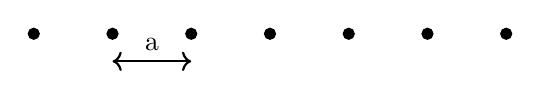
\begin{tikzpicture}
		\filldraw [black]	(0,0.35) circle (2pt)
							(1,0.35) circle (2pt)
							(2,0.35) circle (2pt)
							(3,0.35) circle (2pt)
							(4,0.35) circle (2pt)
							(5,0.35) circle (2pt)
							(6,0.35) circle (2pt);
		\draw [<->, black, thick]	(1, 0) to ["a"] (2, 0);
	\end{tikzpicture}}

	\vspace{10pt}

	\tcbsidebyside[sidebyside adapt=left, blanker, sidebyside gap=1cm,
               sidebyside align=top seam]{\hspace{150pt}\textit{2D:}}{
	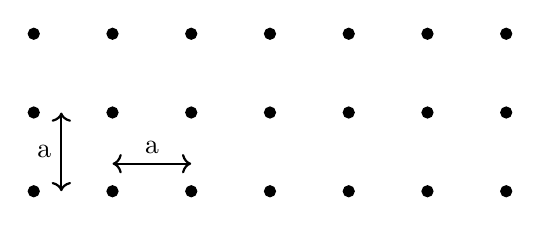
\begin{tikzpicture}
		\filldraw [black]	(0,0) circle (2pt)
							(1,0) circle (2pt)
							(2,0) circle (2pt)
							(3,0) circle (2pt)
							(4,0) circle (2pt)
							(5,0) circle (2pt)
							(6,0) circle (2pt)
							(0,1) circle (2pt)
							(1,1) circle (2pt)
							(2,1) circle (2pt)
							(3,1) circle (2pt)
							(4,1) circle (2pt)
							(5,1) circle (2pt)
							(6,1) circle (2pt)
							(0,2) circle (2pt)
							(1,2) circle (2pt)
							(2,2) circle (2pt)
							(3,2) circle (2pt)
							(4,2) circle (2pt)
							(5,2) circle (2pt)
							(6,2) circle (2pt);
		\draw [<->, black, thick]	(1, 0.35) to ["a"] (2, 0.35);
		\draw [<->, black, thick]	(0.35, 0) to ["a"] (0.35, 1);
	\end{tikzpicture}}

	\vspace{10pt}

	\tcbsidebyside[sidebyside adapt=left, blanker, sidebyside gap=1cm,
               sidebyside align=top seam]{\hspace{150pt}\textit{3D:}}{
	\begin{tikzpicture}
		%	Bottom front
		\draw [*-, black]	(0, 0) to (1, 0);
		\filldraw [black]	(1, 0) circle (2pt);
		\draw [-*, black]	(1, 0) to (2, 0);

		%	Top front
		\draw [*-, black]	(0, 1) to (1, 1);
		\filldraw [black]	(1, 1) circle (2pt);
		\draw [-*, black]	(1, 1) to (2, 1);

		%	Horzontal front
		\draw[--, black]	(0.1, 0) to (0.1, 1)
							(1, 0) to (1, 1)
							(1.9, 0) to (1.9, 1);

		%	Top oblique
		\draw[-*, black]	(0.1, 1) to (0.65, 1.5);
		\draw[-*, black]	(1, 1) to (1.55, 1.5);
		\draw[-*, black]	(1.9, 1) to (2.45, 1.5);

		%	Side right
		\draw[-*, black]	(2.4, 1.5) to (2.4, 0.4);
		\draw[--, black]	(1.9, 0) to (2.4, 0.5);

		%	Top back
		\draw[--, black]	(0.6, 1.45) to (2.4, 1.45);

		%	Inside
		\draw[dotted, black]	(0.1, 0) to (0.6, 0.5)
								(0.6, 0.5) to (2.4, 0.5)
								(0.6, 0.5) to (0.6, 1.5)
								(1.5, 0.5) to (1, 0)
								(1.5, 1.5) to (1.5, 0.5);
		\filldraw[black]	(0.6, 0.5) circle (1pt)
							(1.5, 0.5) circle (1pt);

 		\draw [<->, black, thick]	(1, -0.3) to node [below] {a} (1.9, -0.3);
 		\draw [<->, black, thick]	(2.7, 0.5) to node [right] {a} (2.7, 1.5);
 		\draw [<->, black, thick]	(2.1, -0.1) to node [right=1.2mm, below=0.01mm] {a} (2.6, 0.4);
	\end{tikzpicture}}
	\caption{Lattices in different dimensions}
	\label{fig:lattices}
\end{figure}

As we can probably see, we can always define a some minimal set of vectors that describe the lattice. That means we can indeed go to each lattice point by taking a linear combination of these vectors. An example is given in figure \ref{fig:example_lattice}. \textit{More examples can be found in the slides.} More on lattice vectors in \ref{sec:lattice_vectors}.
\ex{Graphene}{
To show what a lattice is and what it isn't this example is given, see also figure \ref{fig:graphene_lattices}. As we know, graphene has a honeycomb lattice. That's why we call it a honneycomb crystal. But the lattice we can define is called a triangular lattice. Why?\\ \newline
By the definition of a lattice, we must have the same surrounding for every lattice point. This is not the case if we take one atom as basis. Therefore we take a set of two atoms to form the basis and define the lattice point as the center. This results in an equivalent surrounding for every basis structure. \\ \newline
Later on we will define a unit cell (section \ref{sec:unit_cell}) and a conventional unit cell (section \ref{sec:conv_unit_cell}) for this lattice.
}
\begin{figure}[h]
	\centering
	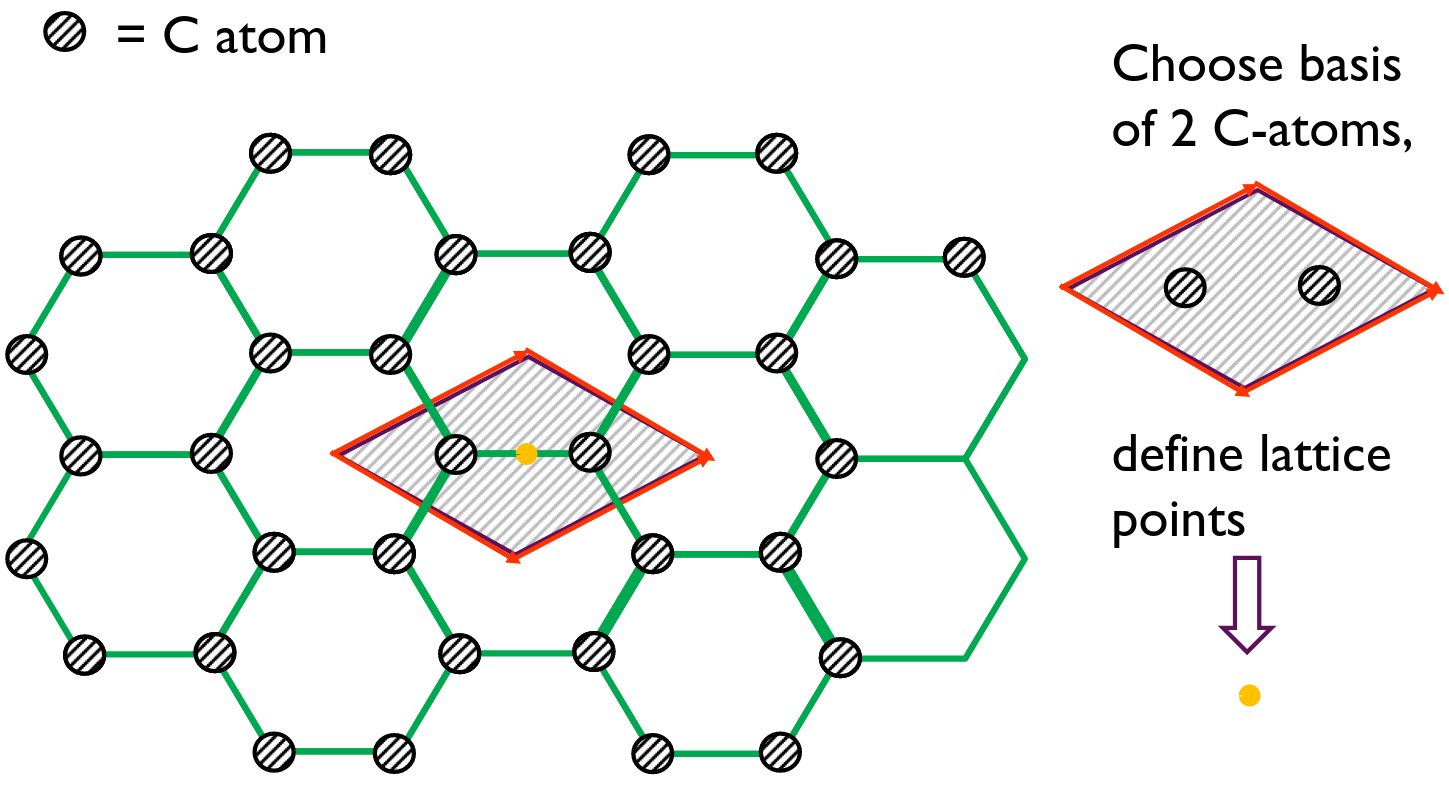
\includegraphics[width=\textwidth/2]{./graphene_lattice}
	\caption{The graphene crystal}
	\label{fig:graphene_lattices}
\end{figure}

\section{Lattice vectors} \label{sec:lattice_vectors}
As already touched upon at section \ref{sec:crystals}, we can define a set of lattice vectors. To construct these we first define an origin O:
\begin{equation}
	O = \vec{0}
\end{equation}
Then we will define the lattice points in function of the PLV \textit{(Primitive Lattice Vectors)}.
\begin{align}
	\vec{a} &= PLV \\
	n_i &\in \bbZ \\
	A &= [\vec{a}_1, \vec{a}_2(, \vec{a}_3)]^T \\
	1D &: \qquad \vec{R} = n_1 \cdot \vec{a} \\
	2D &: \qquad \vec{R} = [n_1, n_2] \cdot A \\
	3D &: \qquad \vec{R} = [n_1, n_2, n_3] \cdot A
\end{align}

We can understand that a lattice must be defined unambiguous, therefore the definition of a lattice can be defined as:
\dfn{Lattice (2)}{A lattice is a set of points defined by Primitive Lattice Vectors (PLV).}
Visually we can represent these vectors as can be seen in figure \ref{fig:example_1Dlattice} and figure \ref{fig:example_lattice}. We can also conclude that \textit{PLV}s are not unique, one can also show that this is true for 3D. These are indeed \textit{PLV}s because one can reach all lattice points.
\begin{figure}[h]
	\centering
	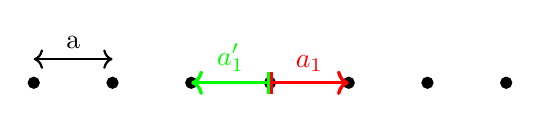
\begin{tikzpicture}
		\filldraw [black]	(0, 0) circle (2pt)
							(1, 0) circle (2pt)
							(2, 0) circle (2pt)
							(3, 0) circle (2pt)
							(4, 0) circle (2pt)
							(5, 0) circle (2pt)
							(6, 0) circle (2pt);
		\draw [|->, red, very thick]	(3, 0) to node [above]{$a_1$} (4, 0);
		\draw [|->, green, very thick]	(3, 0) to node [above]{$a_1'$} (2, 0);

		\draw [<->, black, thick]	(0, 0.3) to node [above]{a} (1, 0.3);
	\end{tikzpicture}
	\caption{An example set of lattice vectors in 1D}
	\label{fig:example_1Dlattice}
\end{figure}
\begin{figure}[h]
	\centering
	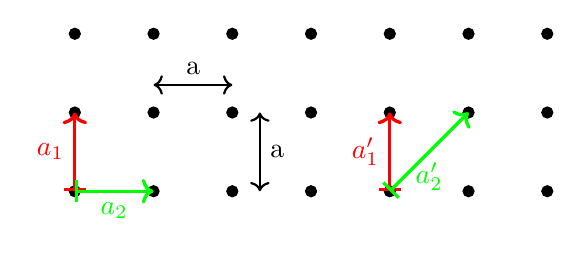
\begin{tikzpicture}
		\filldraw [black]	(0,0) circle (2pt)
							(1,0) circle (2pt)
							(2,0) circle (2pt)
							(3,0) circle (2pt)
							(4,0) circle (2pt)
							(5,0) circle (2pt)
							(6,0) circle (2pt)
							(0,1) circle (2pt)
							(1,1) circle (2pt)
							(2,1) circle (2pt)
							(3,1) circle (2pt)
							(4,1) circle (2pt)
							(5,1) circle (2pt)
							(6,1) circle (2pt)
							(0,2) circle (2pt)
							(1,2) circle (2pt)
							(2,2) circle (2pt)
							(3,2) circle (2pt)
							(4,2) circle (2pt)
							(5,2) circle (2pt)
							(6,2) circle (2pt);
		\draw [<->, black, thick]	(1, 1.35) to ["a"] (2, 1.35);
		\draw [<->, black, thick]	(2.35, 0) to node [right]{a} (2.35, 1);

		\draw [|->, red, very thick]	(0, 0) to node [left]{$a_1$} (0, 1);
		\draw [|->, green, very thick]	(0, 0) to node [below]{$a_2$}(1, 0);

		\draw [|->, red, very thick]	(4, 0) to node [left]{$a_1'$} (4, 1);
		\draw [|->, green, very thick]	(4, 0) to node [below]{$a_2'$}(5, 1);
	\end{tikzpicture}
	\caption{An example set of lattice vectors in 2D}
	\label{fig:example_lattice}
\end{figure}

\section{Unit cell} \label{sec:unit_cell}
\dfn{Unit cell}{A unit cell is a region of space such taht when translated through the entire space by means of lattice vecotrs, reproduces the lattice without any overlaps or voids.}
The definition of a unit cell is illustrated in figure \ref{fig:unit_cell}
\begin{figure}[h]
	\centering
	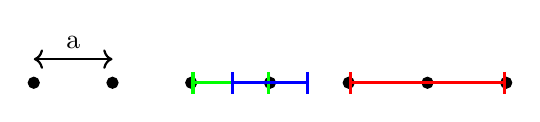
\begin{tikzpicture}
		\filldraw [black]	(0,0) circle (2pt)
							(1,0) circle (2pt)
							(2,0) circle (2pt)
							(3,0) circle (2pt)
							(4,0) circle (2pt)
							(5,0) circle (2pt)
							(6,0) circle (2pt);

		\draw [<->, black , thick]	(0, 0.3) to node [above]{a} (1, 0.3);

		\draw [|-|, green , very thick]	(2, 0) to (3, 0);
		\draw [|-|, red , very thick]	(4, 0) to (6, 0);
		\draw [|-|, blue , very thick]	(2.5, 0) to (3.5, 0);
	\end{tikzpicture}
	\caption{Several 1D unit cells}
	\label{fig:unit_cell}
\end{figure}

\section{Primitive unit cell} \label{sec:prim_unit_cell}


\section{Conventional unit cell} \label{sec:conv_unit_cell}
\dfn{Convetional unit cell}{A convenctional unit cell, a.k.a. a convinient unit cell, is a unit cell that contains mare than 1 lattice point but has perpendicular axis.}
\section{Weigner-Seitz unit cell} \label{sec:weig_cell}
d

\chapter{Periodic Structure of Crystals}
\section{Bravais lattices}
\dfn{Bravais latticees}{There are 14 different lattice types, these are called Bravais lattices. These lattices can be subdivided into 7 different lattice systems, these lattice systems are:
\begin{enumerate}
    \setlength\itemsep{0pt}
    \item   Triclinic
    \item   Monoclinic
    \item   Orthohombric
    \item   Tetragonal
    \item   Cubic
    \item   Triagonal
    \item   Hexagonal
\end{enumerate}
The Cubic structure will mostly be studied during this course.
}

\section{Cubic lattice systems}
Cubic lattice systems come in three flavours, we will define them here. The different systems can be found in figure \ref{fig:cubic_lattice_systems}.
\begin{figure}
    \centering
    \begin{tikzpicture}
		%	Bottom front
		\filldraw [black]	(0, 0) circle (2pt);
		\draw [-*, black]	(0, 0) to (1, 0);

		%	Top front
		\filldraw [black]	(0, 1) circle (2pt);
		\draw [-*, black]	(0, 1) to (1, 1);

		%	Horzontal front
		\draw[--, black]	(0, 0) to (0, 1)
							(0.9, 0) to (0.9, 1);

		%	Top oblique
		\draw[-*, black]	(0, 1) to (0.55, 1.5);
		\draw[-*, black]	(0.9, 1) to (1.45, 1.5);

		%	Side right
		\draw[-*, black]	(1.4, 1.5) to (1.4, 0.4);
		\draw[--, black]	(0.9, 0) to (1.4, 0.5);

		%	Top back
		\draw[--, black]	(0.4, 1.45) to (1.4, 1.45);

		%	Inside
		\draw[dotted, black]	(0.5, 0.5) to (1.4, 0.5)
                                (0.5, 0.5) to (0, 0)
								(0.5, 1.5) to (0.5, 0.5);
		\filldraw[black]	(0.5, 0.5) circle (1pt);

 		\draw [<->, black, thick]	(0, -0.3) to node [below] {a} (0.9, -0.3);
 		\draw [<->, black, thick]	(1.7, 0.5) to node [right] {a} (1.7, 1.5);
 		\draw [<->, black, thick]	(1.1, -0.1) to node [below=1mm] {a} (1.6, 0.4);
	\end{tikzpicture}
%
	\begin{tikzpicture}
		%	Bottom front
		\filldraw [black]	(0, 0) circle (2pt);
		\draw [-*, black]	(0, 0) to (1, 0);

		%	Top front
		\filldraw [black]	(0, 1) circle (2pt);
		\draw [-*, black]	(0, 1) to (1, 1);

		%	Horzontal front
		\draw[--, black]	(0, 0) to (0, 1)
							(0.9, 0) to (0.9, 1);

		%	Top oblique
		\draw[-*, black]	(0, 1) to (0.55, 1.5);
		\draw[-*, black]	(0.9, 1) to (1.45, 1.5);

		%	Side right
		\draw[-*, black]	(1.4, 1.5) to (1.4, 0.4);
		\draw[--, black]	(0.9, 0) to (1.4, 0.5);

		%	Top back
		\draw[--, black]	(0.4, 1.45) to (1.4, 1.45);

		%	Inside
		\draw[dotted, black]	(0.5, 0.5) to (1.4, 0.5)
                                (0.5, 0.5) to (0, 0)
								(0.5, 1.5) to (0.5, 0.5);
		\filldraw[black]	(0.5, 0.5) circle (1pt);

		% Body centering
		\filldraw [gray] (0.7, 0.7) circle (2pt);

 		\draw [<->, black, thick]	(0, -0.3) to node [below] {a} (0.9, -0.3);
 		\draw [<->, black, thick]	(1.7, 0.5) to node [right] {a} (1.7, 1.5);
 		\draw [<->, black, thick]	(1.1, -0.1) to node [below=1mm] {a} (1.6, 0.4);
	\end{tikzpicture}
%
	\begin{tikzpicture}
		%	Face centering
		\filldraw [gray]	(0.95, 0.95) circle (2pt);

		%	Bottom front
		\filldraw [black]	(0, 0) circle (2pt);
		\draw [-*, black]	(0, 0) to (1, 0);

		%	Top front
		\filldraw [black]	(0, 1) circle (2pt);
		\draw [-*, black]	(0, 1) to (1, 1);

		%	Horzontal front
		\draw[--, black]	(0, 0) to (0, 1)
							(0.9, 0) to (0.9, 1);

		%	Top oblique
		\draw[-*, black]	(0, 1) to (0.55, 1.5);
		\draw[-*, black]	(0.9, 1) to (1.45, 1.5);

		%	Side right
		\draw[-*, black]	(1.4, 1.5) to (1.4, 0.4);
		\draw[--, black]	(0.9, 0) to (1.4, 0.5);

		%	Top back
		\draw[--, black]	(0.4, 1.45) to (1.4, 1.45);

		%	Inside
		\draw[dotted, black]	(0.5, 0.5) to (1.4, 0.5)
                                (0.5, 0.5) to (0, 0)
								(0.5, 1.5) to (0.5, 0.5);
		\filldraw[black]	(0.5, 0.5) circle (1pt);

		% Face centering
		\filldraw [gray]	(0.5, 0.5) circle (2pt)
							(0.25, 0.75) circle (2pt)
							(0.7, 1.25) circle (2pt)
 							(0.7, 0.25) circle (2pt)
 							(1.15, 0.7) circle (2pt);

 		\draw [<->, black, thick]	(0, -0.3) to node [below] {a} (0.9, -0.3);
 		\draw [<->, black, thick]	(1.7, 0.5) to node [right] {a} (1.7, 1.5);
 		\draw [<->, black, thick]	(1.1, -0.1) to node [below=1mm] {a} (1.6, 0.4);
	\end{tikzpicture}
    \caption{The three different cubic lattice systems}
    \label{fig:cubic_lattice_systems}
\end{figure}
\dfn{Simple cubic lattice}{A simple cubic lattice is a conventional unit cell and therefore also a \textit{PUC}. This lattice has a straightforward basis, as can be seen in figure \ref{fig:simple_cubic_lattice}.}
The basis chosen is $\{\vec{a}_1, \vec{a}_2, \vec{a}_3\}$. As we can see (figure \ref{fig:simple_cubic_lattice}), the basis isn't body centered. Because the body centered atom is a different one as the other 'side' atoms, the smallest possible unit cell (or \textit{PUC}) is the full cube. Whereas if the middle atom is the same, the basis is chosen in the middle, this is the \textbf{body centered cubic lattice}.
\begin{figure}[h]
    \centering
    \begin{tikzpicture}
		%	Bottom front
		\filldraw [black]	(0, 0) circle (2pt);
		\draw [-*, black]	(0, 0) to (1, 0);

		%	Top front
		\filldraw [black]	(0, 1) circle (2pt);
		\draw [-*, black]	(0, 1) to (1, 1);

		%	Horzontal front
		\draw[--, black]	(0, 0) to (0, 1)
							(0.9, 0) to (0.9, 1);

		%	Top oblique
		\draw[-*, black]	(0, 1) to (0.55, 1.5);
		\draw[-*, black]	(0.9, 1) to (1.45, 1.5);

		%	Side right
		\draw[-*, black]	(1.4, 1.5) to (1.4, 0.4);
		\draw[--, black]	(0.9, 0) to (1.4, 0.5);

		%	Top back
		\draw[--, black]	(0.4, 1.45) to (1.4, 1.45);

		%	Inside
		\draw[dotted, black]	(0.5, 0.5) to (1.4, 0.5)
                                (0.5, 0.5) to (0, 0)
								(0.5, 1.5) to (0.5, 0.5);
		\filldraw[black]	(0.5, 0.5) circle (1pt);

		% Body centering
		\filldraw [cyan] (0.7, 0.7) circle (2pt);

		\draw [->, cyan, thin]	(0.7, 0.7) to node [right=9mm]{different atom} (2.4, 0.7);

 		\draw [<->, black, thick]	(0, -0.3) to node [below] {a} (0.9, -0.3);
 		\draw [<->, black, thick]	(1.7, 0.5) to node [right] {a} (1.7, 1.5);
 		\draw [<->, black, thick]	(1.1, -0.1) to node [below=1mm] {a} (1.6, 0.4);

 		%	Basis
 		\draw [|->, green, very thick]	(0, 0) to (0.9, 0);
 		\draw [|->, red, very thick]	(0, 0) to (0, 1);
 		\draw [|->, blue, very thick]	(0, 0) to (0.48, 0.48);
	\end{tikzpicture}
	\caption{The basis for a simple cubic lattice}
	\label{fig:simple_cubic_lattice}
\end{figure}

\dfn{Body centered cubic lattice}{A Body centered cubic lattice has 1 atom as primitive unit cell, its basis is depectied in figure \ref{fig:bodycubic_lattice_system}. As mentioned before, all atoms are the same and that is why the \textit{PUC} is smaller.}
\begin{figure}[h]
    \centering
	\begin{tikzpicture}
		%	Bottom front
		\filldraw [black]	(0, 0) circle (2pt);
		\draw [-*, black]	(0, 0) to (1, 0);

		%	Top front
		\filldraw [black]	(0, 1) circle (2pt);
		\draw [-*, black]	(0, 1) to (1, 1);

		%	Horzontal front
		\draw[--, black]	(0, 0) to (0, 1)
							(0.9, 0) to (0.9, 1);

		%	Top oblique
		\draw[-*, black]	(0, 1) to (0.55, 1.5);
		\draw[-*, black]	(0.9, 1) to (1.45, 1.5);

		%	Side right
		\draw[-*, black]	(1.4, 1.5) to (1.4, 0.4);
		\draw[--, black]	(0.9, 0) to (1.4, 0.5);

		%	Top back
		\draw[--, black]	(0.4, 1.45) to (1.4, 1.45);

		%	Inside
		\draw[dotted, black]	(0.5, 0.5) to (1.4, 0.5)
                                (0.5, 0.5) to (0, 0)
								(0.5, 1.5) to (0.5, 0.5);
		\filldraw[black]	(0.5, 0.5) circle (1pt);

		% Body centering
		\filldraw [gray] (0.7, 0.7) circle (2pt);

 		\draw [<->, black, thick]	(0, -0.3) to node [below] {a} (0.9, -0.3);
 		\draw [<->, black, thick]	(1.7, 0.5) to node [right] {a} (1.7, 1.5);
 		\draw [<->, black, thick]	(1.1, -0.1) to node [below=1mm] {a} (1.6, 0.4);

 		%	Basis
 		\draw [|->, green, very thick]	(0.7, 0.7) to (0.05, 0.05);
 		\draw [|->, red, very thick]	(0.7, 0.7) to (1.4, 0.5);
 		\draw [|->, blue, very thick]	(0.7, 0.7) to (1, 1);
	\end{tikzpicture}
    \caption{The three different cubic lattice systems}
    \label{fig:bodycubic_lattice_system}
\end{figure}

\dfn{Face centered cubic lattice}{If all atoms are the same and the extra atoms position themselves on the middle of every face, one gets the face centere cubic lattice. This is depicted in figure \ref{fig:facecubic_lattice_system}.}
\begin{figure}[h]
    \centering
	\begin{tikzpicture}
		%	Face centering
		\filldraw [gray]	(0.95, 0.95) circle (2pt);

		%	Bottom front
		\filldraw [black]	(0, 0) circle (2pt);
		\draw [-*, black]	(0, 0) to (1, 0);

		%	Top front
		\filldraw [black]	(0, 1) circle (2pt);
		\draw [-*, black]	(0, 1) to (1, 1);

		%	Horzontal front
		\draw[--, black]	(0, 0) to (0, 1)
							(0.9, 0) to (0.9, 1);

		%	Top oblique
		\draw[-*, black]	(0, 1) to (0.55, 1.5);
		\draw[-*, black]	(0.9, 1) to (1.45, 1.5);

		%	Side right
		\draw[-*, black]	(1.4, 1.5) to (1.4, 0.4);
		\draw[--, black]	(0.9, 0) to (1.4, 0.5);

		%	Top back
		\draw[--, black]	(0.4, 1.45) to (1.4, 1.45);

		%	Inside
		\draw[dotted, black]	(0.5, 0.5) to (1.4, 0.5)
                                (0.5, 0.5) to (0, 0)
								(0.5, 1.5) to (0.5, 0.5);
		\filldraw[black]	(0.5, 0.5) circle (1pt);

		% Face centering
		\filldraw [gray]	(0.5, 0.5) circle (2pt)
							(0.25, 0.75) circle (2pt)
							(0.7, 1.25) circle (2pt)
 							(0.7, 0.25) circle (2pt)
 							(1.15, 0.7) circle (2pt);

 		\draw [<->, black, thick]	(0, -0.3) to node [below] {a} (0.9, -0.3);
 		\draw [<->, black, thick]	(1.7, 0.5) to node [right] {a} (1.7, 1.5);
 		\draw [<->, black, thick]	(1.1, -0.1) to node [below=1mm] {a} (1.6, 0.4);

 		%	Basis
 		\draw [|->, red, very thick]	(0, 0) to (0.25, 0.75);
 		\draw [|->, blue, very thick]	(0, 0) to (0.7, 0.25);
		\draw [|->, green, very thick]	(0, 0) to (0.5, 0.5);
	\end{tikzpicture}
    \caption{The three different cubic lattice systems}
    \label{fig:facecubic_lattice_system}
\end{figure}

\section{C/Si/Ge - lattice systems}
As we know, the lattice systems for C, Si and Ge have a diamond lattice structre. This diamond structure takes the form of a fcc (face centered cubic) lattice.

\chapter{Reciprocal Space}
\section{Definition and properties}
\dfn{Direction}{The direction in reciprocal space is defined by [$u, v, w$]}
\dfn{Planes}{The reciprocal planes are defined by ($h, k, l$)}
\clm{Properties of reciprocal space}{}{
\begin{enumerate}
    \setlength\itemsep{0pt}
    \item There are an infinite amount of lattice planes in a lattice.
    \item The set of all lattice planes contains only parallel lattice plains that contain all lattice points.
    \item The lattice plane closest to the origin cuts the coordinate axis in ($\frac{1}{h}, \frac{1}{k}, \frac{1}{l}$).
    \item There is always a lattice plane going through the origin.
\end{enumerate}
}

\section{Reciprocal space} \label{sec:reciproc_space}
\subsection{Fourier transform of a periodic function}
As we know from section \ref{sec:trans_symm}, $V(\vec{r})$ is periodic. That's why we look at the FT of a periodic function.
\begin{align}
    f(x)    &= f(x + n\cdot a) \\
            &= \frac{a_0}{2} + \sum_{n=2}^{\infty}\left\{a_n\cos\frac{2\pi \cdot nx}{a} + b_n\sin\frac{2\pi \cdot nx}{a}\right\}\\
            &= \sum_{G}^{}{F(G)\cdot e^{iGx}}
\end{align}
Assuming for $n= -\infty \rightarrow \infty$
\begin{align}
    G &= \frac{2\pi}{a}n \\
    G\cdot a &= 2n\pi \\
    &\Rightarrow e^{iGa} = e^{2\pi n i} = 1
\end{align} \nt{For a reciporcal lattice number G: $[G] = \frac{1}{2}$}
Furthermore, the solutions for $a_n$ and $b_n$ are give by:
\begin{align}
    a_n &= \frac{2}{a_0} \int_{0}^{a} dx f(x)\cos\frac{2\pi \cdot nx}{a}\\
    b_n &= \frac{2}{a_0} \int_{0}^{a} dx f(x)\sin\frac{2\pi \cdot nx}{a}
\end{align}
\clm{Property of $F(G)$}{}{For a real sum: $F(-G) = F^*(G)$}
\qs{Using the FT for conversion of the lattice space to the recipocal space}{How does this translate to the lattice and potential?}
\ex{Using the FT for conversion of the lattice space to the recipocal space}{
	\tcbsidebyside[sidebyside adapt=center, blanker, sidebyside gap=-12cm,
               sidebyside align=middle]{\textit{1D:}}
	{
		\tcbsidebyside[sidebyside adapt=left, blanker, sidebyside gap=1cm,
				sidebyside align=top seam]{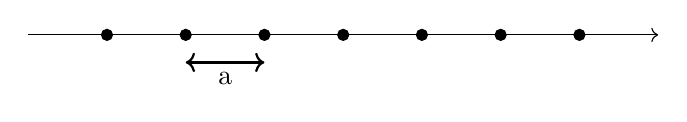
\begin{tikzpicture}
				\filldraw [black]	(0,0.35) circle (2pt)
									(1,0.35) circle (2pt)
									(2,0.35) circle (2pt)
									(3,0.35) circle (2pt)
									(4,0.35) circle (2pt)
									(5,0.35) circle (2pt)
									(6,0.35) circle (2pt);
				\draw [<->, black, thick]	(1, 0) to node [below]{a} (2, 0);
				\draw [->, black] (-1, 0.35) to (7, 0.35);
			\end{tikzpicture}}{\hspace{5pt}\textit{x}}

		\vspace{10pt}

		\tcbsidebyside[sidebyside adapt=left, blanker, sidebyside gap=1cm,
				sidebyside align=top seam]{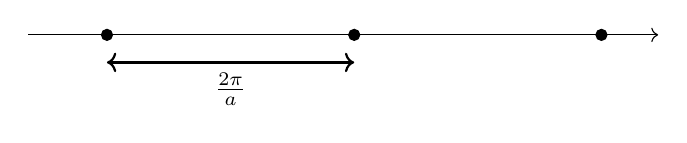
\begin{tikzpicture}
				\filldraw [black]	(0,0.35) circle (2pt)
									(3.14,0.35) circle (2pt)
									(6.28,0.35) circle (2pt);
				\draw [<->, black, thick]	(0, 0) to node[below]{$\frac{2\pi}{a}$} (3.14, 0);
				\draw [->, black] (-1, 0.35) to (7, 0.35);
			\end{tikzpicture}}{\hspace{5pt}\textit{k}}
	}
	In lattice space we see that $V(x)$ is periode, $V(x) = V(x + na)$. $a$ is the lattice vector.
}
\subsection{Extension to 2D/3D}
Now, extending the above principle to 2D and 3D is straightforward but I'll still go over it.
\thm{}{
\begin{align}
	f(\vec{r}) &= f(x, y, z) = f(\vec{r} + \vec{T})\\
	&\Rightarrow e^{i\vec{G}\cdot\vec{T}} = 1 \qquad \forall \vec{T}
\end{align}

We define $\vec{r}$ as a vector in the lattice space and $\vec{T} = n_1\cdot\vec{a}_1 + n_2\cdot\vec{a}_2 + n_3\cdot\vec{a}_3$.
}
\begin{myproof}
\begin{align}
	f(\vec{r}) = \sum_{\vec{G}}^{}{&F(\vec{G})e^{i\vec{G}\cdot\vec{r}}} &\\
	\Rightarrow f(\vec{r} + \vec{T}) &= \sum_{\vec{G}}^{}{F{\vec{G}}e^i\vec{G}\cdot(\vec{r} + \vec{T})}\\
	&= \sum_{\vec{G}}^{}{F{\vec{G}}e^i\vec{G}\cdot(\vec{r})}\\
	e^{i\vec{G}\cdot\vec{T}} &= 1
\end{align}
\end{myproof}
By section \ref{sec:trans_symm} we can do step ($3.13$) because we know $f(\vec{r}) = f(\vec{r} + \vec{T})$ for a periodic lattice.
In general we can say: \begin{equation} F(\vec{G}) = \frac{1}{V}\int_{V}^{}f(\vec{r})e^{-i\vec{G}\cdot\vec{r}}d\vec{r} \end{equation}.

\section{Finding reciprocal lattice vectors}
As we know is $\vec{G}$ the reciprocal lattice vector, but how do we find this vector?\\
We know that: \begin{equation} e^{i\vec{G}\cdot\vec{T}} = 1 \Rightarrow \vec{G}\cdot\vec{T} = 2\pi n \label{eqn:def_of_G}\end{equation}
With
\begin{align}
	\vec{G} &= m_1\cdot\vec{b}_1 + m_2\cdot\vec{b}_2 + m_3\cdot\vec{b}_3 \\
	\vec{T} &= n_1\cdot\vec{a}_1 + n_2\cdot\vec{a}_2 + n_3\cdot\vec{a}_3 \\
	n &\rightarrow \delta_{ij} = \left\{
		\begin{array}{lr}
			1 & \text{if } i = j \\
			0 & \text{if } i \neq j
		\end{array}
	\right\label{eqn:deltarelation}
\end{align}
This results in the following definition: \begin{equation} \vec{a}_i \cdot \vec{b}_j = 2\pi\delta_{ij} \end{equation}
\nt{The reason for defining $\delta_{ij}$ as either $0$ or $1$ is to have orthogonal $\vec{a}_i$ and $\vec{b}_j$.}
Then the following vectors $\vec{b}_j$ span the reciprocal space $\vec{G}$. When satisfying relation ($3.20$), $\vec{b}_j$ can be described in function of $\vec{a}_i$:
\begin{align}
	\vec{b}_1 &= 2\pi\frac{\vec{a}_2\times\vec{a}_3}{\vec{a}_1\cdot(\vec{a}_2\times\vec{a}_3)} = \frac{2\pi}{V}(\vec{a}_2\times\vec{a}_3) \label{eqn:b1}\\
	\vec{b}_2 &= 2\pi\frac{\vec{a}_3\times\vec{a}_1}{\vec{a}_2\cdot(\vec{a}_3\times\vec{a}_1)} = \frac{2\pi}{V}(\vec{a}_3\times\vec{a}_1)\\
	\vec{b}_3 &= 2\pi\frac{\vec{a}_1\times\vec{a}_2}{\vec{a}_3\cdot(\vec{a}_1\times\vec{a}_2)} = \frac{2\pi}{V}(\vec{a}_1\times\vec{a}_2) \label{eqn:b3}\\
	&\Rightarrow \vec{G} = m_1\cdot\vec{b}_1 + m_2\cdot\vec{b}_2 + m_3\cdot\vec{b}_3
\end{align}
As we see describing $\vec{b}_j$ is a cyclic procedure.

\section{Properties of reciporcal spaces}
\clm{Property 1}{}{To every lattice plane ($h, k, l$) there is a reciprocal lattice vector perpendicular to that plane and is given by $\vec{G} = h\cdot\vec{b}_1 + k\cdot\vec{b}_2 + l\cdot\vec{b}_3$.}
\begin{myproof}
	It is sufficient to show that the vector $\vec{R}$, perpendicular to the lattice plan ($h, k, l$), is parallel to $\vec{G}$. In order that: \begin{equation} \frac{\vec{R}}{\norm{\vec{R}}} = \frac{\vec{G}}{\norm{\vec{G}}} \end{equation}
	Then take a lattice plane ($h, k, l$):
	\begin{center}
	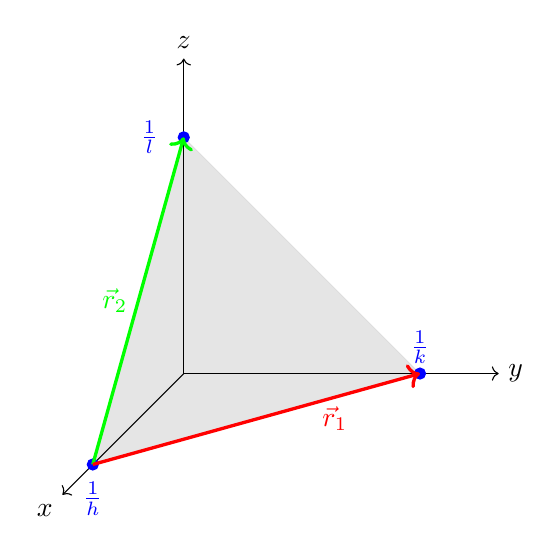
\begin{tikzpicture}
		\draw [->, black]	(0, 0, 0) to (0, 0, 4) node[anchor=north east]{$x$};
		\draw [->, black]	(0, 0, 0) to (0, 4, 0) node[above]{$z$};
		\draw [->, black]	(0, 0, 0) to (4, 0, 0) node[right]{$y$};

		\filldraw[draw=gray, opacity=0.1] (0, 0, 3) to (0, 3, 0) to (3, 0, 0);

		\filldraw[blue]	(0, 0, 3) circle (2pt);
		\filldraw[blue]	(0, 3, 0) circle (2pt);
		\filldraw[blue]	(3, 0, 0) circle (2pt);

		\draw [->, green, very thick]	(0, 0, 3) to node[left]{$\vec{r}_2$} (0, 3, 0);
		\draw [->, red, very thick]	(0, 0, 3) to node[right=7mm]{$\vec{r}_1$} (3, 0, 0);

		\draw [blue] (0, 3, 0) node[left=2mm] {$\frac{1}{l}$};
		\draw [blue] (3, 0, 0) node[above] {$\frac{1}{k}$};
		\draw [blue] (0, 0, 3) node[below=1mm] {$\frac{1}{h}$};
	\end{tikzpicture}
	\end{center}
	We define $\vec{r}_1 = \frac{\vec{a}_2}{k} - \frac{\vec{a}_1}{h}$ and $\vec{r}_2 = \frac{\vec{a}_3}{l} - \frac{\vec{a}_1}{h}$.
	The vector perpendiculas to the area spanned (gray) by $\vec{r}_1$ and $\vec{r}_2$ is given by $\vec{R} = \vec{r}_1 \times \vec{r}_2$. If we fill in the vectors according to the definitons, we get:
	\begin{align}
		\vec{R} &= \left\{\frac{\vec{a}_2}{k} - \frac{\vec{a}_1}{h}\right\} \times \left\{\frac{\vec{a}_3}{l} - \frac{\vec{a}_1}{h}\right\} \\
		&= \frac{\vec{a}_2}{k} \times \left\{\frac{\vec{a}_3}{l} - \frac{\vec{a}_1}{h} \right\} - \frac{\vec{a}_1}{h} \times \left\{\frac{\vec{a}_3}{l} - \frac{\vec{a}_1}{h} \right\} \label{eqn:determinant_R}\\
		&= C\cdot\vec{G} \\
		&\sim \vec{G}
	\end{align}

	And thus from
		\begin{align}
		\frac{\vec{G}}{\norm{\vec{G}}} &= \frac{\vec{R}}{\norm{\vec{R}}} \\
		&= \frac{C\cdot\vec{G}}{\norm{C\cdot\vec{G}}} \\
		&= \frac{C\cdot\vec{G}}{C\cdot\norm{\vec{G}}} = \frac{\vec{G}}{\norm{\vec{G}}}\\
		&\Rightarrow \vec{R} // \vec{G}\nonumber
		\end{align}
\end{myproof}
\nt{If you work out equation \ref{eqn:determinant_R} you get the formulas for $\vec{b}_j$, see equations \ref{eqn:b1} - \ref{eqn:b3}. Keep in mind that $\vec{a} \times -\vec{b} = \vec{b} \times \vec{a}$ and that distributivity is defined for cross products.}

\clm{Property 2}{}{The spacing d between the lattice plane closest to the origin and the origin itself is given by:
\begin{align}
	&\frac{2\pi}{\norm{\vec{G}}} \\
	\Rightarrow \norm{\vec{G}} &= \frac{2\pi}{d} \label{eqn:braggplane_distande}
\end{align}}
\begin{myproof}
\begin{align}
	d &= \text{the distance betwee the ($h, k, l$) planes} \nonumber \\
	&= \frac{\vec{a}_1}{h}\cdot\frac{\vec{G}}{\norm{\vec{G}}} \\
	&= \frac{1}{h\norm{\vec{G}}}h\vec{a}_1\cdot\vec{b}_1 = \frac{2\pi}{\norm{\vec{G}}} \label{eqn:prop2simplification}
\end{align}
Step \ref{eqn:prop2simplification} uses the fact that $\vec{a}_i$ and $\vec{b}_j$ are perpendicular as per \ref{eqn:deltarelation}.
\end{myproof}

\clm{Property 3}{}{The direct lattice is the reciprocal of its own reciprocal lattice. Because switching the vectors in expression \ref{eqn:def_of_G} results in the same expression.}

\clm{Property 4}{}{The volume of a primitive unit cell of the reciprocal lattice is given by:
\begin{align}
	V_R &= \vec{b}_1\cdot(\vec{b}_2\times\vec{b}_3) \\
	&= \frac{8\pi^3}{V}
\end{align}
With $V = \vec{a}_1\cdot(\vec{a}_2\times\vec{a}_3)$, the volume of the direct lattice \textit{PUC}.}

\section{X-ray diffraction}
One way where the 'Von Laue-Bragg' condition can be observed is in x-ray diffraction. The 'Von Laue-Bragg' condition states that an inciding electron is or scattered or stays unscattered when colliding with a crystal. This scattering is elastic thus the amplitude of the wave function does not change. This is illustrated in figure \ref{fig:vonlaue}.
\begin{figure}[b]
    \centering
    \begin{tikzpicture}
        \draw[->, black]	node[left] {$e^-$}(0, 0) to node[above]{incident} node[below]{$\vec{k}$} (2, 0);

        \draw[black] plot [smooth cycle] coordinates {(2.6, 0) (3.2, 0.6) (2.9, 0.7) (3.5, 1) (4.2, 0.9) (4.5, -0.3) (3.9, -0.2) (3.5, -0.7)} node [above=5mm, size=1pt]{CRYSTAL};

        \draw[->, black]	(5, 0.2) to node[above]{$\vec{k}'$}(6, 0.8) node[right=1mm]{$e^-$ (scattered)};
		\draw[->, black]	(5, 0) to node[below]{$\vec{k}$}(6, 0) node[right=1mm]{$e^-$ (unscattered)};
    \end{tikzpicture}
    \caption{X-ray diffraction on a lattice}
    \label{fig:vonlaue}
\end{figure}
Becuase the scattering is elastic we can state the following, define the wave as $e^{i\vec{k}\cdot\vec{r}}$:
\begin{align}
	E(\vec{k}) &= \frac{\hbar^2k^2}{2m}\\
	&= E(\vec{k}')\\
	&= \frac{\hbar^2k'^2}{2m}\\
	&\Rightarrow \abs{\vec{k}} = \abs{\vec{k}'}
\end{align}
One way of figuring out if an electron is scattered is to use the Fermi golden rule.
\section{Fermi golden rule}
abc

\subsection{Von Laue-Bragg condition} \label{sec:bragg}
abc

\section{Von Laue-Bragg condition}
abc

\section{The Brillouin Zone (BZ)} \label{sec:Brillouin}
abc

\chapter{Solids}
\section{Defining solids}
\qs{What is a solid?}{Solid = nuclei + electrons}
For describing solids we define following concepts:
\dfn{Core electrons}{
	\begin{itemize}
		\setlength\itemsep{0pt}
		\item Tightly bound to nucleus
		\item Occupy lower shells
		\item Do not participate in bonding
	\end{itemize}}
\dfn{Valence electrons}{
	\begin{itemize}
		\setlength\itemsep{0pt}
		\item Loosely bound to nucleus
		\item Occupy higher E-shells
		\item Responsible for bonding
	\end{itemize}}

To describe the Hamiltonian for solids for the Schödinger equation we use:
\begin{align}
	H &= H_{electron} + H_{electron - electron} + H_{nucleus} + H_{nucleus - nuclues} + H_{electron - nucleus} \\
	H &= H_{electron} + H_{electron - electron} + H_{ion} + H_{ion - ion} + H_{electron - ion}
\end{align} \par
The following definitions for the $H_{i}$ are used:
\begin{gather}
	H_{electron} = \sum_{i = 1}^{N}{-\frac{\hbar^2}{2m_{electron}} \nabla_i^2}\\
	H_{nucleus} = \sum_{i = 1}^{M}{-\frac{\hbar^2}{2*M_i} \nabla_o^2}\\
	H_{electron - electron} = \frac{1}{2} \sum_{i, j; i \neq j}^{}{\frac{e^2}{4 \pi \epsilon_0 \abs{\vec{r}_i - \vec{r}_j}}}\\
	H_{nucleus - nucleus} = \frac{1}{2} \sum_{i, j; i \neq j}^{}{\frac{Z_i Z_j e^2}{4 \pi \epsilon_0 \abs{\vec{R}_i - \vec{R}_j}}}\\
	H_{electron - nucleus} = \sum_{i, j}^{}{-\frac{Z_j e^2}{4 \pi \epsilon_0 \abs{\vec{r}_i - \vec{R}_j}}}
\end{gather}

%% next page

\nt{In equation $(1.5)$ and $(1.11)$ we have $i \neq j$ in order that we do not double count $i$.\\ Furthermore, in equation $(1.8)$ and we have $Z_i$ which is an atomic number}
To further describe the solid lattice, one has to describe ions. In essence, ions are just nuclei and core electrons together. In the following equations is $ M' = M $ and the amount of valence electrons is $ N' $.\\ \par
Looking at the hamiltonians of the electron - ion interactions, these become:
\begin{gather}
	H_{electron} = \sum_{i = 1}^{N'}{-\frac{\hbar^2}{2m_{electron}} \nabla_i^2}\\
	H_{ion} = \sum_{i = 1}^{M'}{-\frac{\hbar^2}{2*M_i} \nabla_o^2}\\
	H_{electron - electron} = \frac{1}{2} \sum_{i, j; i \neq j}^{}{\frac{e^2}{4 \pi \epsilon_0 \abs{\vec{r}_i - \vec{r}_j}}}\\
	H_{ion - ion} = \frac{1}{2} \sum_{i, j; i \neq j}^{}{V_{ion}(\vec{R}_i - \vec{R}_j)}\\
	H_{electron - ion} = \sum_{i, j}^{}{V_{electron - ion}(\vec{r}_i - \vec{R}_j)}
\end{gather} \par
We can see the equations for electron - ion interactions are very similar to electron nucleus interactions. \\ \par

What we eventually want to solve is: $ H\Phi = E\Phi $. We will therefore define following vectors: \\$\vec{r} = (\vec{r}_1, \vec{r}_2, \dots, \vec{r}_N)$ and $\vec{R} = (\vec{R}_1, \vec{R}_2, \dots, \vec{R}_M)$. \\
We can now define the probability density function as: $P (\vec{r}, \vec{R}) = \abs{\Phi(\vec{r}, \vec{R})}^2$
Later on, we separate the degrees of freedom of valence electrons from the degrees of freedom of bound electrons, that's why we separated them here already.

\section{Born-oppenheimer approximation}
This definition comes down to saying electrons move much faster as ions thus ions are immobile.
\begin{equation}
	H\Phi(\vec{r}, \vec{R}) = E\Phi(\vec{r}, \vec{R})
\end{equation}
\clm{}{}{$ \Phi(\vec{r}, \vec{R}) \approx \psi(\vec{r}, \vec{R})\phi(\vec{R}) $}
\begin{align}
	H\Phi(\vec{r}, \vec{R}) & = H\psi(\vec{r}, \vec{R})\phi(\vec{R}) \\
	& = (H_{electron} + H_{electron - electron} + H_{ion} + H_{ion - ion} + H_{electron - ion})\psi(\vec{r}, \vec{R})\phi(\vec{R}) \\
	& = (H_{electron} + H_{electron - electron} + H_{electron - ion})\psi(\vec{r}, \vec{R})\phi(\vec{R}) + (H_{ion} + H_{ion - ion})\psi(\vec{r}, \vec{R})\phi(\vec{R}) \\
	& = \phi(\vec{R})(H_{electron} + H_{electron - electron} + H_{electron - ion})\psi(\vec{r}, \vec{R}) + \psi(\vec{r}, \vec{R})(H_{ion} + H_{ion - ion})\phi(\vec{R}) \nonumber \\
	& \qquad + (H_{ion} + H_{ion - ion})\psi(\vec{r}, \vec{R})\phi(\vec{R}) - \psi(\vec{r}, \vec{R})(H_{ion} + H_{ion - ion})\phi(\vec{R})
\end{align}

We can move $\phi(\vec{R})$ to the front because there is no differnetial operation acting on it in the hamiltonians.\\
In step 3 we perform a `+ $\psi(\vec{r}, \vec{R})(H_{ion} + H_{ion - ion})\phi(\vec{R})$' and `- $\psi(\vec{r}, \vec{R})(H_{ion} + H_{ion - ion})\phi(\vec{R})$' operation. \par
Because $m_{electron} \approx M \cdot 10^-4$, $(H_{ion} + H_{ion - ion})\psi(\vec{r}, \vec{R})\phi(\vec{R}) - \psi(\vec{r}, \vec{R})(H_{ion} + H_{ion - ion})\phi(\vec{R}) \approx 0$.
We can now simplify equation $ (1.5) = E\psi(\vec{r}, \vec{R})\phi(\vec{R}) $ further by dividing with $ \psi(\vec{r}, \vec{R})\phi(\vec{R}) $. \\
Equation $(1.5)$ now becomes:
\begin{equation}
	\frac{(H_{electron} + H_{electron - electron} + H_{electron - ion})\psi(\vec{r}, \vec{R})}{\psi(\vec{r}, \vec{R})} + \frac{(H_{ion} + H_{ion - ion})\phi(\vec{R})}{\phi(\vec{R})} = E
\end{equation}
\nt{We cannot divide the leftover function as the numerator still acts on it!} \par
We can now define:
\begin{equation}
	E_{el}(\vec{R}) = E - \frac{(H_{ion} + H_{ion - ion})\phi(\vec{R})}{\phi(\vec{R})}
\end{equation}
As mentioned before already, this makes it possible to separate valence electronic part and the ionic part.
\dfn{Formulation of the solid hamiltonians}{
	\begin{equation}
		\left\{\begin{align}
		(H_{electron} + H_{electron - electron} + H_{electron - ion})\psi(\vec{r}, \vec{R}) &= E_{el}\psi(\vec{r}, \vec{R})\\
		\frac{(H_{ion} + H_{ion - ion})\phi(\vec{R})}{\phi(\vec{R})}\psi(\vec{r}, \vec{R}) &= (E - E_{el})\psi(\vec{r}, \vec{R})
		\end{align}\right.
	\end{equation}
}
\section{Static approximation (w.r.t. the lattic)}
We know $\vec{R} = (\vec{R}_1, \vec{R}_2, \dots, \vec{R}_M) => \vec{R}^{(0)}_i + \delta\vec{R}_i(t)$ This delta is small and can be ignored.
\begin{align}
	H_{electron - ion} & = \sum{V_{electron - ion}(\vec{r}_i - \vec{R}_j)} \\
	& = \sum{(V_{electrion - ion}(\vec{r}_i - \vec{R}^{(0)}_j) + \delta\vec{R}_j(t) \cdot \vec{\nabla}_j V_{electrion - ion}(\vec{r}_i - \vec{R}^{(0)}_j))}
\end{align}
\nt{
	\begin{itemize}
	\item $\delta\vec{R}_j(t) \cdot \vec{\nabla}_j V_{electrion - ion}(\vec{r}_i - \vec{R}^{(0)}_j)$ is the electron - phonon interaction.
	\item Why does it only depend on distance? In normal curcomstances, most interactions are distance related but sometimes it is (in anisotropic materials) vector dependent, therefore the $\abs{}$ is left out here in $H_{electron - ion}$.
	\end{itemize}
}
Now we simplify equation $(1.20)$, in hope for writing the time dependent Schrödinger equation easier. Namely it becomes a signle electron particle operator istead of a complex Hamiltonian.
\begin{itemize}
	\setlength\itemsep{0mm}
	\item $H_{electron}$ stays the same
	\item $H_{electrion - ion}$ stays the same
	\item $H_{electron - electron} = 1/2 \sum{\frac{e^2}{4 \pi \epsilon_0 \abs{\vec{r}_i - \vec{r}_j}}} \approx \sum{v_i(\vec{r}_i)}$
\end{itemize}
Such that:
\begin{align}
	& \sum_{i}^{}{\left\{-\frac{\hbar^2}{2m_{electron}} \nabla_i^2 + \sum_{j}^{}{\left\{V_{electron - ion}(\vec{r}_i- \vec{R}_j) + v_i(\vec{r}_i)\right\}}\right\}}\psi(\vec{r}, \vec{R}) = E_{el}\psi(\vec{r}, \vec{R}) \\
	& \Rightarrow \sum{h_i(\vec{r}_i)}\psi(\vec{r}) = E_{el}\psi(\vec{r}) \\
	& \qquad \qquad \longrightarrow \psi(\vec{r}) = \xi(\vec{r}_1) + \xi(\vec{r}_2) + \dots \\
	& \Rightarrow h_i(r_i)\xi(\vec{r}_i) = \epsilon_i \xi(\vec{r}_i)
\end{align}

\section{Hartree approximation}
\qs{What does this approximation mean?}{
	First of all, the Hartree approximation is an electron - electron interaction approximation.
	It means that electron number $i$ sees all other electrons as a continious charge distribution.
	\begin{align}
		& g_i(\vec{r}) = \sum_{k \neq i}^{}{-e \abs{\xi_k(\vec{r})}^2} \\
		& \qquad \qquad \longrightarrow \nabla^2\Phi_i(\vec{r}) = \frac{g_i(\vec{r})}{\epsilon}
	\end{align}
}
We can calculate the Potential enegery as follows:
\begin{align}
	v_i(\vec{r}) &= -e \Phi \\
	&= \sum_{k \neq i}^{}{\int_{V}^{}{\frac{e^2 \abs{\xi_k(\vec{r})}^2}{4\pi \epsilon_0 \abs{\vec{r} - \vec{r}'}}dr'}}
\end{align}
\nt{$\Phi$ is electrostatic potential. Furthermore, $\vec{r}_i$ means it \textbf{belongs} to electron i.}

Now we can solve the one electron problem by:
\begin{align}
	& h(\vec{r})\xi(\vec{r}) = \epsilon \xi(\vec{r}) \\
	\Rightarrow & \quad h(\vec{r}) = -\frac{\hbar^2}{2m_e}\nabla^2 + v(\vec{r}) + \sum{V_{electron - ion}(\vec{r} - \vec{R})}
\end{align}
\par Looking at the last part of $h$ we see that in a lattice, $\vec{R}$ is a lattice vector. Then for a solid, the lattice is infinite and therefore $V_{electron - ion}$ will be periodic.
We will call $\sum{V_{electron - ion}(\vec{r} - \vec{R})}$ a periodic potential: $U(\vec{r}) = U(\vec{r} - \vec{R}_l')$ \\ \par
\cor{Conslusion}{As show above we can now write the Schrödinger equation as a simplified wave function:
	\begin{equation}
		\left(-\frac{\hbar^2}{2m_e}\nabla^2 + V(\vec{r})\right)\xi(\vec{r}_i) = \epsilon \xi(\vec{r}_i)
	\end{equation}
}


\chapter{Band Theory of Metals}
In Chapter \ref{ch:solids}, we showed how all the contributions of all the valence ions/electrons/..., kinetic energies and interactions between the particles could be written as a one electron Schrödinger equation. Some approximations made to achieve this are: Born-Oppenheimer apporximation, Hartree approximation and the static approximation.
The one electron Schrödinger equation states:
\begin{equation}
	\left[-\frac{\hbar^2}{2m}\nabla^2 + V(\vec{r})\right]\psi(\vec{r}) = E\psi(\vec{r}) \label{eqn:schrodinger_tbu}
\end{equation}
As we know, this potential is called the crystal potential energy fucntion. It has periodic properties. Now, we can deduce properties, originating from the periodicity of $V(\vec{r})$, af this Schrödinger equation.

\section{Property 1: Influence of translation operator on the Schrödinger equation} \label{sec:property1}
\dfn{Translation operator}{What is a translation operator: \begin{equation} \hat{T}_{\vec{R}}f(\vec{r}) = f(\vec{r} + \vec{R}) \end{equation}}
\nt{We put a hat ( $\hat{}$ ) on the letter to show that it is a operator.}
Applying this on the Schrödinger equation result in:
\begin{align}
	\hat{T}_{\vec{R}}H\psi(\vec{r}) &= \hat{T}_{\vec{R}}(H(\vec{r})\psi(\vec{r}))\\
	&= H(\vec{r} + \vec{R})\psi(\vec{r} + \vec{R})\\
	&= H(\vec{r})\psi(\vec{r} + \vec{R})\\
	&= H(\vec{r})\hat{T}_{\vec{R}}\psi(\vec{r})
\end{align}
Thus we can conclude that:
\begin{align}
	\hat{T}_{\vec{R}}H\psi &= H\hat{T}_{\vec{R}}\psi \\
	\hat{T}_{\vec{R}}H &= H\hat{T}_{\vec{R}} \\
	\left[\hat{T}_{\vec{R}}, H\right] &= 0 \label{eqn:commutation}
\end{align}
\clm{Product of translation operators}{}{The product of two translation operators can be defined as: \begin{equation} \hat{T}_{\vec{R}}\hat{T}_{\vec{R}'} = \hat{T}_{\vec{R} + \vec{R}'}  \label{prop:translation} \end{equation}}
\begin{myproof}
	We can show this by simply working out the operations on a function:
	\begin{align}
		\hat{T}_{\vec{R}}\hat{T}_{\vec{R}'}\psi(\vec{r}) &= \hat{T}_{\vec{R}}\psi(\vec{r} + \vec{R}') \\
		&= \psi(\vec{r} + \vec{R} + \vec{R}') \\
		&= \hat{T}_{\vec{R} + \vec{R}'}\psi(\vec{r})
	\end{align}
\end{myproof}
What is now so interesting about this commutation relation (equation \ref{eqn:commutation})? Well, it is linked to a fundamental property of Quantum mechanics.
\thm{Property of commutators in QM}{If $\left[\hat{T}_{\vec{R}}, H\right] = 0$ then all eigenstates of $H$ can be chosen to have the same eigenstates as $\hat{T}_{\vec{R}}$. In other words, if $H$ and $\hat{T}_{\vec{R}}$ commute, than they have a commen set of eigenstates. We will derive them here.\par
Because the translational operator has the same set of eigenstates the following set of equations are equivalent.
\begin{align}
	\left\{
	\begin{array}{lr}
		H\psi = E\psi \\
		\hat{T}_{\vec{R}}\psi = \lambda(\vec{R})\psi
	\end{array}
	\right
\end{align}
We still do not know what these $\lambda(\vec{R})$ eigenvalues belong to it, the energy states are the same.\par
Following from the property form equation \ref{prop:translation}, we can deduce some properties for $\lambda(\vec{R})$:
\begin{align}
	& \lambda(\vec{R})\lambda(\vec{R}') = \lambda(\vec{R} + \vec{R}') \\
	& \lambda^n(\vec{R}) = \lambda(n\vec{R})
\end{align}
A value that satisfies, these two conditions is:
\begin{equation}
	\lambda(\vec{R}) = e^{i\vec{k}\cdot\vec{R}} \qquad \text{with $\vec{k}$ some complex vector.}
\end{equation}
Normalisation requires that:
\begin{align}
	\int_{V}^{}\abs{\psi}^2d\vec{r} &= 1 \label{eqn:norm} \\
	\Rightarrow \int_{V}^{}\abs{\hat{T}_{\vec{R}}\psi(\vec{r})}^2d\vec{r} &= \int_{V}^{}\abs{\psi(\vec{r} + \vec{R})}^2d\vec{r} \label{eqn:norm_2} \\
	&= \int_{V}^{}\abs{\lambda(\vec{R})\psi(\vec{r})}^2d\vec{r} \nonumber \\
	&= \int_{V}^{}\abs{\lambda(\vec{R})}^2\abs{\psi(\vec{r})}^2d\vec{r} \nonumber\\
	&= \abs{\lambda(\vec{R})}^2\int_{V}^{}\abs{\psi(\vec{r})}^2d\vec{r} \nonumber \\
	&= \abs{\lambda(\vec{R})}^2 \label{eqn:simplification_integral}  \\
	&= 1 \label{eqn:lambda_simplification}
\end{align}
Step \ref{eqn:simplification_integral} is possible due to \ref{eqn:norm}. The last step (equation \ref{eqn:lambda_simplification}) follows from that is $\psi$ is normalized (equation \ref{eqn:norm}), the translation of $\psi$ is still normalized.\par
Now because of the fact that we have the normalisation (equation \ref{eqn:norm_2}), we can say that $\vec{k}$ can be written as a real vector $k_x\vec{e}_x + k_y\vec{e}_y + k_z\vec{e}_z$ with $k \in \bbR$.\par
Now because we have a periodic crystal potential, we can write the following:
\begin{equation}
	\hat{T}_{\vec{R}}\psi(\vec{r}) = e^{i\vec{k}\cdot\vec{R}}\psi(\vec{r}) \label{eqn:eigenstates_transoperator}
\end{equation}}

\section{Bloch's theorem} \label{sec:bloch}
\dfn{Block's theorem}{The Bloch's theorem states:
\begin{equation}
	\psi(\vec{r}) = u(\vec{r})e^{i\vec{k}\cdot\vec{r}} \qquad \text{where } u(\vec{r}) \text{ is periodic}
\end{equation}
$e^{i\vec{k}\cdot\vec{r}}$ is a plain wave function.}
\ex{How Bloch's theorem works}{
	\begin{align}
		\hat{T}_{\vec{R}}\psi(\vec{r}) &= \hat{T}_{\vec{R}}\left(u(\vec{r})e^{i\vec{k}\cdot\vec{r}}\right) \\
		&= u(\vec{r} + \vec{R})e^{i\vec{k}\cdot(\vec{r} + \vec{R})} \\
		\text{(if }u(\vec{r})\text{ is periodic)}\qquad &= e^{i\vec{k}\cdot(\vec{r} + \vec{R})}u(\vec{r}) \\
		\text{(using Bloch)}\qquad &= e^{i\vec{k}\cdot\vec{R}}\psi(\vec{r}) \\
		&= \lambda(\vec{R})\psi(\vec{r}) \\
		&= \hat{T}_{\vec{R}}\psi(\vec{r})
	\end{align}
}

Furthermore, you can the eigenstates of the translation operator (equation \ref{eqn:eigenstates_transoperator}), too:
\begin{equation}
	\hat{T}_{\vec{R}}\psi(\vec{r}) = \psi(\vec{r} + \vec{R}) = u(\vec{r} + \vec{R})e^{i\vec{k}\cdot(\vec{r} + \vec{R})} = u(\vec{r})e^{i\vec{k}\cdot\vec{r}}e^{i\vec{k}\cdot\vec{R}} = e^{i\vec{k}\cdot\vec{R}}\psi(\vec{r})
\end{equation}

\subsection{Closer look at the Schrödinger equation}
To identify each wavevector, we will use a $\vec{k}$ subscript referring to the plain wave in Bloch's theorem (section \ref{sec:bloch}). As it turns out the function $u(\vec{r})$ will also depend on $\vec{k}$ ($u_{\vec{k}}(\vec{r})$). We now get the following by using Bloch:
\begin{align}
	H\psi &= E\psi \\
	H\psi_{\vec{k}}(\vec{r}) &= E(\vec{k})\psi_{\vec{k}}(\vec{k})\\
	\left\{\frac{\hbar^2}{2m}\left(-i\vec{\nabla}+ \vec{k}\right)^2 + V(\vec{r})\right\}u_{\vec{k}}(\vec{r}) &= E(\vec{k})u_{\vec{k}}(\vec{r}) \label{eqn:eigvalprob}
\end{align}
We get a Schrödinger equation for the periodic function $u$. Equation \ref{eqn:eigvalprob} is an eigenvalue problem that is confined in a finite volume (the cyrstal) where $u$ has to obey to it's periodic boundary conditions $u_{\vec{k}}(\vec{r}) = u_{\vec{k}}(\vec{r} + \vec{R})$. What are the eigenvalues?\par
From differential equation analysis and eigenvalue problems we know we get a discrete set of eigenvalues: $E_n(\vec{k})$. This existence of this discrete set is because we impose boundary conditions on the problem. We can now 'update' the Schrödinger equation (\ref{eqn:eigvalprob}):
\begin{equation}
	\left\{\frac{\hbar^2}{2m}\left(-i\vec{\nabla}+ \vec{k}\right)^2 + V(\vec{r})\right\}u_{n, \vec{k}}(\vec{r}) &= E(n, \vec{k})u_{n, \vec{k}}(\vec{r}) \label{eqn:schrodinger_complete}
\end{equation}

\section{Properties of the energy eigenvalues of $u_{n, \vec{k}}$}
\clm{}{}{Both wave function and energy eigenvalues satisfy (for $\vec{G}$ a reciprocal lattice vector):
\begin{equation}
	\left\{
	\begin{array}{lr}
		E_n(\vec{k} + \vec{G}) = E_n(\vec{k}) \\
		\psi_{n, \vec{k} + \vec{G}}(\vec{r}) = \psi_{n, \vec{k}}(\vec{r})
	\end{array}
	\right
\end{equation}}
\begin{myproof}
	If we substitude the following equation into equation \ref{eqn:schrodinger_tbu}, we get \ref{eqn:updatedschrod}.
	\begin{equation}
		\psi_{n, \vec{k} + \vec{G}}(\vec{r}) = u_{n, \vec{k} + \vec{G}}(\vec{r})e^{i(\vec{k} + \vec{G})\cdot\vec{r}}
	\end{equation}
	\begin{equation}
		\left\{\frac{\hbar^2}{2m}\left(-i\vec{\nabla} + \vec{k}\right)^2 + V(\vec{r})\right\}u_{n, \vec{k} + \vec{G}}(\vec{r})e^{i\vec{G}\cdot\vec{r}} = E_n(\vec{k} + \vec{G})u_{n, \vec{k} + \vec{G}}(\vec{r})e^{i\vec{G}\cdot\vec{r}} \label{eqn:updatedschrod}
	\end{equation}
	What we see now is that from \ref{eqn:schrodinger_complete} and \ref{eqn:updatedschrod} we expect:
	\begin{equation}
		u_{n, \vec{k} + \vec{G}}(\vec{r})e^{i\vec{G}\cdot\vec{r}} = u_{n, \vec{k}}(\vec{r})
	\end{equation}
	Thereby we can say that:
	\begin{equation}
		\psi_{n, \vec{k} + \vec{G}}(\vec{r}) = u_{n, \vec{k} + \vec{G}}(\vec{r})e^{i(\vec{k} + \vec{G})\cdot\vec{r}} = u_{n, \vec{k} + \vec{G}}(\vec{r})e^{i\vec{k}\cdot\vec{r}} = \psi_{n, \vec{k}}(\vec{r})
	\end{equation}
	Now we can also show that $E_n(\vec{k} + \vec{G}) = E_n(\vec{k})$.
\end{myproof}
What you might notice now is that $\vec{G}$ can be any vector, instead of being a reciprocal lattice vector. How do we enforce this requirement? Well, because equation \ref{eqn:schrodinger_complete} and equation \ref{eqn:updatedschrod} are the same, the wavefunctions must obey the same periodic boundary conditions. That is only true if $\vec{G}$ is a reciprocal lattice vector.
We can show this has to be the case by:
\begin{align}
	\hat{T}_{\vec{R}}\left(u_{n, \vec{k} + \vec{G}}(\vec{r})e^{i\vec{G}\cdot\vec{r}}\right) &= u_{n, \vec{k} + \vec{G}}(\vec{r} + \vec{R})e^{i\vec{G}\cdot(\vec{r} + \vec{R})} \\
	&= u_{n, \vec{k} + \vec{G}}(\vec{r})e^{i\vec{G}\cdot\vec{r}}e^{i\vec{G}\cdot\vec{R}} \\
	&\Rightarrow e^{i\vec{G}\cdot\vec{R}} = 1
\end{align}

\section{Property 2: Inversion symmetry} \label{sec:property2}
\dfn{Inversion symmetry}{Inversion symmetry states that \begin{equation} E_n(-\vec{k}) = E_n(\vec{k}) \label{eqn:property2} \end{equation}}
This has an effect on a property of the wave equation:
\begin{align}
	\psi_{n, \vec{k}}^{*}(\vec{r} + \vec{R}) &= \left(\psi_{n, \vec{k}}(\vec{r} + \vec{R})\right)^{*} \\
	\text{(By equation \ref{eqn:eigenstates_transoperator})}\qquad &= \left(e^{i\vec{k}\cdot\vec{R}}\psi_{n, \vec{k}}(\vec{r})\right)^{*} \\
	&= e^{-i\vec{k}\cdot\vec{R}}\psi_{n, \vec{k}}^{*}(\vec{r})
\end{align}
The complex conjugate wavefunction still complies with Bloch's theorem, therefore we can say that:
\begin{equation}
	\psi_{n, \vec{k}}^{*}(\vec{r}) = \psi_{n, -\vec{k}}(\vec{r})
\end{equation}
Now, we proof the property for energy eigenvalues (equation \ref{eqn:property2}) by starting form the complex conjugate Schrödinger equation:
\begin{align}
	H^{*}\psi_{n, \vec{k}}^{*}(\vec{r}) = H\psi_{n, \vec{k}}^{*}(\vec{r}) &= \left(H\psi_{n, \vec{k}}(\vec{r})\right)^{*} \\
	&= \left(E_n(\vec{k})\psi_{n, \vec{k}}(\vec{r})\right)^{*} \\
	&= E_n\psi_{n, \vec{k}}^{*}(\vec{r}) \\
	\Rightarrow H\psi_{n, -\vec{k}}(\vec{r}) &= E_n(-\vec{k})\psi_{n, -\vec{k}}(\vec{r}) \\
	&= E_n(-\vec{k})\psi_{n, \vec{k}}^{*}(\vec{r}) \\
	\Rightarrow E_n(-\vec{k}) = E_n(\vec{k}) \nonumber
\end{align}

\section{Consequences of the properties}
As we saw for the Schrödinger equation:
\begin{align}
    &-\frac{\hbar^2}{2m}\nabla^2\psi_{n, \vec{k}}(\vec{r}) + V(\vec{r})\psi_{n, \vec{k}}(\vec{r}) = E_n(\vec{k})\psi_{n, \vec{k}}(\vec{r}) \\
    & \qquad \rightarrow V(\vec{r}) = V(\vec{r} + \vec{R})
\end{align}

This says something about the energy spectrum, in function of $\vec{k}$. As we see in figure \ref{fig:energybandiagram}, we have energy bands $E_i$, these all have all eigenvalues and between the bands we have bandgaps, there there aro no eigenvalues. Now there is also a possibility of overlap of the energy bands.\par
\begin{figure}[h]
    \centering
    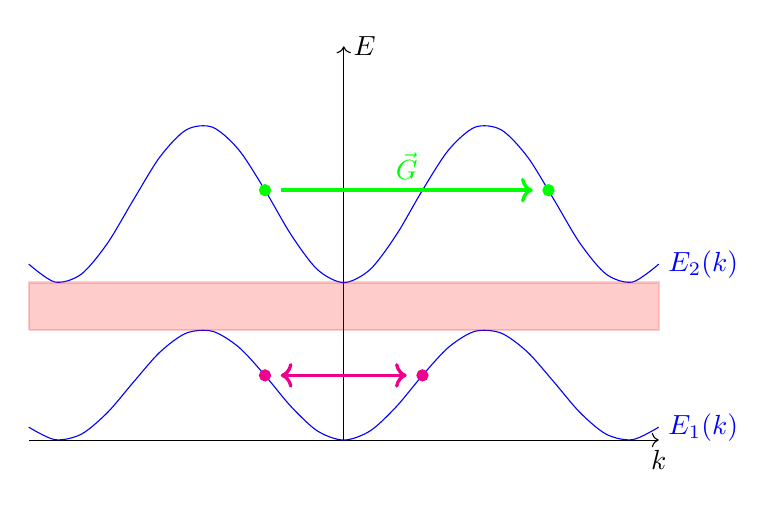
\begin{tikzpicture}
        \draw[->, black] (0, 0) to (0, 5) node[right]{$E$};
        \draw[->, black] (-4, 0) to (4, 0) node[below]{$k$};

        \draw[domain=-4:4, smooth, variable=\x, blue] plot ({\x}, {-0.7*cos(\x*100)+0.7}) node[right]{$E_1(k)$};
        \draw[domain=-4:4, smooth, variable=\x, blue] plot ({\x}, {-cos(\x*100)+3}) node[right]{$E_2(k)$};

        \filldraw[-, draw=red, fill=red, opacity=0.2, thick] (-4, 1.4) to (-4, 2) to (4, 2) to (4, 1.4) to (-4, 1.4);

        \filldraw[green]	(-1, {-cos(-100)+3}) circle (2pt)
							(2.6, {-cos(-100)+3}) circle (2pt);
		\draw[->, green, very thick]	(-0.8, {-cos(-100)+3}) to node[above]{$\vec{G}$} (2.4, {-cos(-100)+3});

		\filldraw[magenta]	(-1, {-0.7*cos(-100)+0.7}) circle (2pt)
							(1, {-0.7*cos(-100)+0.7}) circle (2pt);
		\draw[<->, magenta, very thick]	(-0.8, {-0.7*cos(-100)+0.7}) to (0.8, {-0.7*cos(-100)+0.7});
    \end{tikzpicture}
    \caption{Energy band diagram}
    \label{fig:energybandiagram}
\end{figure}
The wave functions are also periodic in k-space. Thus if we take the green point and translate that on the wave, that point has the same wave, this is translational symmetry (section \ref{sec:property1}). We also notice inversion symmetry, depicted in magenta (section \ref{sec:property2}).

\section{Empty lattice - 1D}
Suppose we take a very trivial example: take $V(x) = 0$, then the Schrödinger equation is very simple to solve. $V(x) = 0$ means we have free electrons.
\begin{align}
    &V(x+a) = V(x) = 0\\
    &-\frac{\hbar^2}{2m}\frac{d^2}{dx^2}\psi_k(x) = E(k)\psi_k(x)\\
    &\psi_k(x) = \frac{1}{\sqrt{L}}e^{ikx} \qquad E(k) = \frac{\hbar^2k^2}{2m} & \text{for }\frac{-G}{2} \leq k \leq \frac{G}{2} \label{eqn:solution}
\end{align}

Equation \ref{eqn:solution} gives the wave functions of the Schrödinger equation, the corresponding energies are solutions of the Schrödinger equation, too. Seen in figure \ref{fig:displacedenergybands}, when we shift our wavefunction and energy with G, we get a periodic energy spectrum. If we plot these extra potentials, we get what we call energy bands on the intersections. For a free particle, this is silly because these bandgaps have $0$ width, yet they are labeled with a gray dot.

\begin{figure}[h]
    \centering
    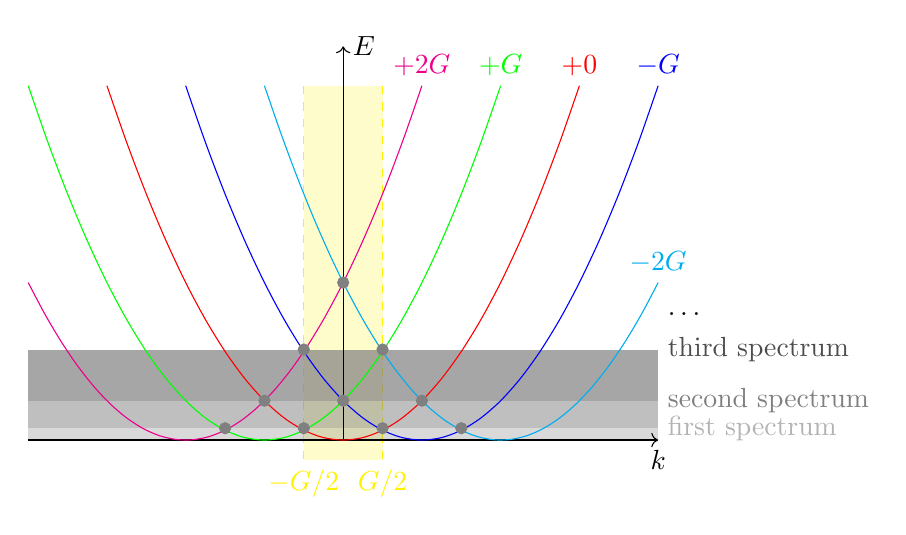
\begin{tikzpicture}
    	\draw[dashed, yellow]	(0.5, 4.5) to (0.5, -0.25) node[below]{$G/2$};
		\draw[dashed, yellow]	(-0.5, 4.5) to (-0.5, -0.25) node[below]{$-G/2$};

		\fill[fill=yellow, opacity=0.2]	(0.5, 4.5) to (0.5, -0.25) to (-0.5, -0.25) to (-0.5, 4.5);
		\fill[fill=gray, opacity=0.3]	(-4, 0.15) to (-4, 0) to (4, 0) to (4, 0.15) node[right]{first spectrum};
		\fill[fill=gray, opacity=0.5]	(-4, 0.15) to (-4, 0.5) to (4, 0.5) node[right]{second spectrum} to (4, 0.15);
		\fill[fill=gray, opacity=0.7]	(-4, 1.15) to (-4, 0.5) to (4, 0.5) to (4, 1.15) node[right]{third spectrum};

		\draw (4, 1.6) node[right]{\dots};

        \draw[->, black] (0, 0) to (0, 5) node[right]{$E$};
        \draw[->, black] (-4, 0) to (4, 0) node[below]{$k$};

		\draw[domain=-3:3, smooth, variable=\x, red] plot ({\x}, {\x*\x/2}) node[above]{$+0$};
		\draw[domain=-4:2, smooth, variable=\x, green] plot ({\x}, {(\x +1)*(\x +1)/2}) node[above]{$+G$};
		\draw[domain=-4:1, smooth, variable=\x, magenta] plot ({\x}, {(\x +2)*(\x +2)/2}) node[above]{$+2G$};
		\draw[domain=-2:4, smooth, variable=\x, blue] plot ({\x}, {(\x -1)*(\x -1)/2}) node[above]{$-G$};
		\draw[domain=-1:4, smooth, variable=\x, cyan] plot ({\x}, {(\x -2)*(\x -2)/2}) node[above]{$-2G$};

		\filldraw[gray]	(-0.5, 0.15) circle (2pt)
						(-1.5, 0.15) circle (2pt)
						(0.5, 0.15) circle (2pt)
						(1.5, 0.15) circle (2pt)
						(-1, 0.5) circle (2pt)
						(0, 0.5) circle (2pt)
						(1, 0.5) circle (2pt)
						(0.5, 1.15) circle (2pt)
						(-0.5, 1.15) circle (2pt)
						(0, 2) circle (2pt);
    \end{tikzpicture}
    \caption{Displaced energy bands with different spectra}
    \label{fig:displacedenergybands}
\end{figure}
\nt{Keep in mind that: $\frac{G}{2} - \frac{-G}{2} = \frac{2\pi}{a}$.}
\section{Nearly free electron-approximation}
Now, we include a weak preiodic potential. Then the hamiltonian becomes:
\begin{equation}
    \hat{H} = \hat{H}_0 + V(\vec{r})
\end{equation}
Where $\hat{H}$ is the free kinetic operator: $-\frac{\hbar^2}{2m}\nabla^2$ and $V(\vec{r})$ is the introduced weak potential.
We can solve it by using the pertrubation theory for solving this modified Schrödinger equation.
First solve Schrödinger for $H_0$, this gives:
\begin{align}
	&\hat{H}_0 \psi^{(0)}_{\vec{k}}(\vec{r}) = E^{(0)}_{\vec{k}} \psi^{(0)}_{\vec{k}}(\vec{r})\\
	&\qquad \Rightarrow \left\{
		\begin{array}{lr}
			\psi^{(0)}_{\vec{k}}(\vec{r}) = \frac{1}{\sqrt{V}}e^{i\vec{k}\cdot\vec{r}}\\
			E^{(0)}(\vec{k}) = \frac{\hbar^2k^2}{2m} \label{eqn:E0}
		\end{array}
	\right
\end{align}

\subsection{Pertrubation theory}
Solving with the weak potential goes as follows:
\begin{align}
    & E(\vec{k}) \approx E^{(0)}(\vec{k}) + E^{(1)}(\vec{k}) + E^{(2)}(\vec{k})\\
    & E^{(0)}(\vec{k}) = \text{ see equation \ref{eqn:E0}}\\
    & E^{(1)}(\vec{k}) =\quad <\vec{k}^{(0)} | V(\vec{r}) | \vec{k}^{(0)}>\quad = \int_{V}^{}\frac{1}{\sqrt{V}}e^{-i\vec{k}\cdot\vec{r}}V(\vec{r}) \frac{1}{\sqrt{V}}e^{i\vec{k}\cdot\vec{r}}V(\vec{r})\\
    & E^{(2)}(\vec{k}) = \sum_{\vec{k}' \neq \vec{k}} \frac{\abs{<\vec{k}^{(0)} | V(\vec{r}) | \vec{k}^{(0)}>}^2}{E^{(0)}(\vec{k}) - E^{(0)}(\vec{k}')} \label{eqn:E2}
\end{align}
\nt{We use \href{https://phys.libretexts.org/Bookshelves/Quantum_Mechanics/Quantum_Physics_(Ackland)/12\%3A_Scattering_in_Three_Dimensions/12.03\%3A_Box_Normalisation_and_Density_of_Final_States}{box normalisation}, thus putting the particle inside a box, then the k space is a sum instead of an integral. Then at the end making it unbox by making the length infinity again, we see that it works. Now, we have a more convienient way for deriving the same thing because be don't have dirac functoins anymore.}

So let's start calculating the first order approximation:
\begin{align}
    E^{(1)}(\vec{k}) &= \frac{1}{V}\int_{V}{}V(\vec{r})d\vec{r} = \tilde{V}(0) = \text{constant}\\
    E^{(2)}(\vec{k}) &= \text{ see equation \ref{eqn:E2}}\\
    \qquad \text{with: } <\vec{k}' | V(\vec{r}) | \vec{k}> \quad &= \frac{1}{V}\int_{V}{}e^{-i\vec{k}'\cdot\vec{r}}V(\vec{r})e^{i\vec{k}\cdot\vec{r}}\\
    & = \frac{1}{V}\int_{V}{}e^{i(\vec{k} - \vec{k}')\cdot\vec{r}}V(\vec{r})d\vec{r} = \tilde{V}(\vec{k} - \vec{k}')\delta_{\vec{k} - \vec{k}', \vec{G}} \label{eqn:four}
\end{align}

We see a fourier transform in equation \ref{eqn:four}, but as we know the potential $V(\vec{r})$ is periodic thus if $\vec{k}$ is not a lattice vector, the integral must be $0$. Now we can simplify the second step (equation \ref{eqn:E2}):
\begin{equation}
    \sum_{\vec{k}' \neq \vec{k}}\frac{\abs{\tilde{V}(\vec{k} - \vec{k}')\delta_{\vec{k} - \vec{k}', \vec{G}}}^2}{E^{(0)}(\vec{k}) - E^{(0)}(\vec{k}')}
\end{equation}

We rewrite this as \begin{equation} \sum_{\vec{G}}{}\frac{\abs{\tilde{V}(\vec{G})}^2}{E^{(0)}(\vec{k}) - E^{(0)}(\vec{k}')} \end{equation} by using $\vec{k} - \vec{k}' = \vec{G}$ (this is just a simple substitution using the Bragg condition (section \ref{sec:bragg}), the $\delta$-function is in this case 1).
Now we can write equation \ref{eqn:E0} in function of the derived values. Using the "normal" symbolic numeric values for the energies, we get:
\begin{equation}
    E(\vec{k}) \approx \frac{\hbar^2k^2}{2m} + \tilde{V}(0) + \frac{2m}{\hbar^2}\sum_{\vec{G}}^{}\frac{\abs{\tilde{V}(\vec{G})}^2}{k^2 - (\vec{k} - \vec{G})^2}
\end{equation}

As we see this gives a problem when the denominator is $0$, for $k^2 = (\vec{k} - \vec{G})^2$. This is the Bragg condition (section \ref{sec:bragg})!
Let's look more closely at that specific case: $E^{(0)}(\vec{k}) = E^{(0)}(\vec{k} - \vec{G})$:
\begin{equation}
\left\{
\begin{array}{lr}
    \psi^{(0)}_{\vec{k}, 1}(\vec{r}) = \frac{1}{\sqrt{V}}e^{i\vec{k}\cdot\vec{r}} & \text{with: }E^{(0)}(\vec{k}) = \frac{\hbar^2k^2}{2m}\\
    \psi^{(0)}_{\vec{k}, 2}(\vec{r}) = \frac{1}{\sqrt{V}}e^{i(\vec{k}-\vec{G})\cdot\vec{r}} & \text{with: } E^{(0)}(\vec{k}) = \frac{\hbar^2k^2}{2m}
\end{array}
\right
\end{equation}
As we can expect, this is true for multiple values for $k$. We have to deal with a degeneracy.
When you have a degeneracy, you have to span a new wavefunction into your Hilbert space, by using a linear combination of your other wavefunctions. This is Degenerate pertrubation theory, we will go over it in section \ref{sec:dpt}.

\subsection{Degenreate pertrubation theory} \label{sec:dpt}
\nt{Only if we have a degeneracy, $k^2 = (\vec{k} - \vec{G})^2$, we do this section!}
We want to find $\bar{\psi}(\vec{r}) = c_1\psi_{\vec{k}, 1} + c_2\psi_{\vec{k}, 2}$, we obtain this solution by by diagonlalizing the Hamiltonian in the new subspace:
\begin{equation}
    \left[
    \begin{array}{lr}
        H_{11} & H_{12}\\
        H_{21} & H_{22}
    \end{array}  \right]
    \left[
    \begin{array}{lr}
    c_1\\
    c_2
    \end{array}\right]
    =
    E\left[\begin{array}{lr}
    c_1\\
    c_2
    \end{array}\right] \label{eqn:hamiltonians}
\end{equation}
We will work out $H_{11}$, the other solutions are given below.
\begin{align}
    H_{11} &= \int_{V}^{}d\vec{r}\psi^*_{\vec{k}, 1}(\vec{r})\hat{H}\psi_{\vec{k}, 1}(\vec{r}) \\
    &= \int_{V}^{}d\vec{r}\frac{1}{\sqrt{V}}e^{-i\vec{k}\cdot\vec{r}}\left(\frac{-\hbar^2}{2m}\nabla^2\right)\frac{1}{\sqrt{V}}e^{i\vec{k}\cdot\vec{r}}\\
    &\qquad\qquad \text{where }\left(\frac{-\hbar^2}{2m}\nabla^2\right)\frac{1}{\sqrt{V}}e^{i\vec{k}\cdot\vec{r}} \text{ is the free energy of an electron: } E^{(0)}(\vec{k})\frac{1}{\sqrt{V}}e^{i\vec{k}\cdot\vec{r}}\nonumber\\
    &= \frac{1}{V} \int_{V}^{}E^{(0)}(\vec{k})d\vec{r} + \tilde{V}(0)\\
    &= E^{(0)}(\vec{k}) + \tilde{V}(0)
\end{align}
Because $\tilde{V}(0)$ is just a constant, we will set it to $0$. The other hamiltonians are:
\begin{align}
    & H_{12} = \tilde{V}(\vec{G}) \\
    & H_{21} = \tilde{V}(-\vec{G}) = \tilde{V}^*(-\vec{G}) \\
    & H_{22} = E^{(0)}(\vec{k} - \vec{G})
\end{align}
Now we solve equation \ref{eqn:hamiltonians} by means of a determinant, then we get:
\begin{align}
    &\left|\begin{array}{lr}
        H_{11} - E & H_{12}\\
        H_{21} & H_{22} - E
    \end{array}\right| = 0\\
    \Rightarrow E_{\pm}(\vec{k}) &= \frac{\hbar^2}{2m^2}\left(k^2 + (\vec{k} - \vec{G})^2\right)^2 \pm \frac{1}{2} \sqrt{ \left( \frac{\hbar^2}{2m} \right)^2 \left(k^2 - (\vec{k}-\vec{G})\right)^2 + 4\abs{\tilde{V}(\vec{G})}^2}
\end{align}
If we take $k^2 = (\vec{k} - \vec{G})^2$ we get $E_\pm(\vec{k}) = \frac{\hbar^2}{2m}k^2 \pm \abs{\tilde{V}(\vec{G})}$ and we can introduce gaps into our state (it still depends on our fourier transform $\tilde{V}$). The height of the introduced bandgab is: \begin{equation}\Delta E = E_+ - E_- = 2\abs{\tilde{V}(\vec{G})} \label{eqn:bandgapsize} \end{equation} \par
Let's look at this from a more practical standpoint. In figure \ref{fig:simpleEdiagram}, we plot $E^{(0)}(\vec{k})$ and one $E^{(0)}(\vec{k} - \vec{G})$, of course there are more curves but his figure is just for illustration.
\begin{figure}
    \centering
    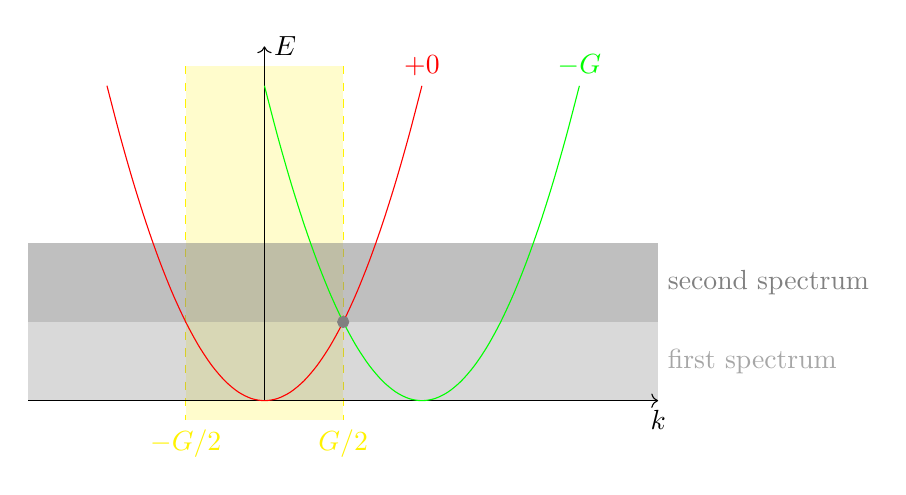
\begin{tikzpicture}
        \draw[dashed, yellow]	(1, 4.25) to (1, -0.25) node[below]{$G/2$};
		\draw[dashed, yellow]	(-1, 4.25) to (-1, -0.25) node[below]{$-G/2$};

		\fill[fill=yellow, opacity=0.2]	(1, 4.25) to (1, -0.25) to (-1, -0.25) to (-1, 4.25);
		\fill[fill=gray, opacity=0.3]	(-3, 1) to (-3, 0) to (5, 0) to (5, 1);
		\draw[gray, opacity=0.7] (5, 0.5) node[right]{first spectrum};
		\fill[fill=gray, opacity=0.5]	(-3, 1) to (-3, 2) to (5, 2) to (5, 1);
		\draw[gray] (5, 1.5) node[right]{second spectrum};
		%\fill[fill=gray, opacity=0.7]	(-3, 1.15) to (-3, 0.5) to (5, 0.5) to (5, 1.15) node[right]{third spectrum};

        \draw[->, black] (0, 0) to (0, 4.5) node[right]{$E$};
        \draw[->, black] (-3, 0) to (5, 0) node[below]{$k$};

		\draw[domain=-2:2, smooth, variable=\x, red] plot ({\x}, {\x*\x}) node[above]{$+0$};
		\draw[domain=0:4, smooth, variable=\x, green] plot ({\x}, {(\x - 2)*(\x - 2)}) node[above]{$-G$};

		\filldraw[gray]	(1, 1) circle (2pt);
    \end{tikzpicture}
    \caption{The simplified energy diagram}
    \label{fig:simpleEdiagram}
\end{figure}
\begin{figure}
    \centering
    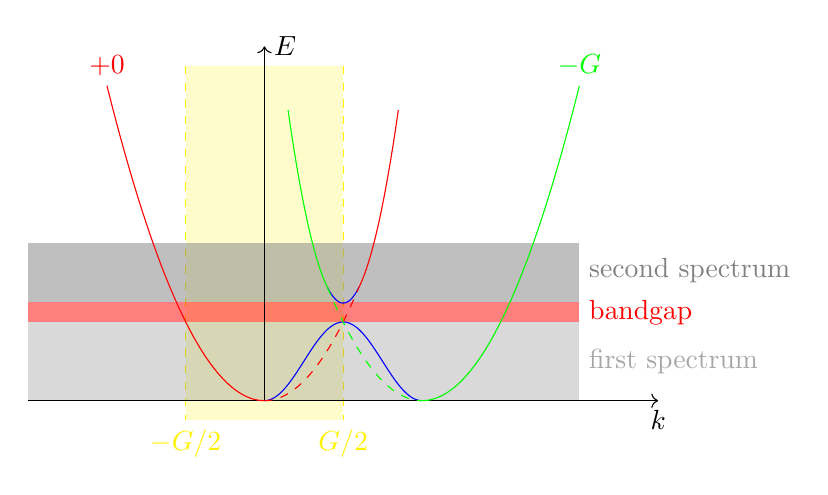
\begin{tikzpicture}
        \draw[dashed, yellow]	(1, 4.25) to (1, -0.25) node[below]{$G/2$};
		\draw[dashed, yellow]	(-1, 4.25) to (-1, -0.25) node[below]{$-G/2$};

		\fill[fill=yellow, opacity=0.2]	(1, 4.25) to (1, -0.25) to (-1, -0.25) to (-1, 4.25);
		\fill[fill=gray, opacity=0.3]	(-3, 1) to (-3, 0) to (4, 0) to (4, 1);
		\draw[gray, opacity=0.7] (4, 0.5) node[right]{first spectrum};
		\fill[fill=gray, opacity=0.5]	(-3, 1.25) to (-3, 2) to (4, 2) to (4, 1.25);
		\draw[gray] (4, 1.65) node[right]{second spectrum};
		\fill[fill=red, opacity=0.5]	(-3, 1) to (-3, 1.25) to (4, 1.25) to (4, 1);
		\draw[red] (4, 1.125) node[right]{bandgap};

        \draw[->, black] (0, 0) to (0, 4.5) node[right]{$E$};
        \draw[->, black] (-3, 0) to (5, 0) node[below]{$k$};

		\draw[domain=-2:0, smooth, variable=\x, red] plot ({\x}, {\x*\x});
		\draw[red] (-2, 4) node[above]{$+0$};
		\draw[domain=0:1, smooth, variable=\x, blue] plot ({\x}, {sin((\x - 1/2)*180)/2+1/2});
		\draw[domain=1:2, smooth, variable=\x, blue] plot ({\x}, {sin((\x - 1/2)*180)/2+1/2});
		\draw[domain=2:4, smooth, variable=\x, green] plot ({\x}, {(\x - 2)*(\x - 2)}) node[above]{$-G$};

		\draw[domain=0.3:0.8, smooth, variable=\x, green] plot ({\x}, {5*(\x - 1.2)*(\x - 0.8) + 1.44});
		\draw[domain=1.2:1.7, smooth, variable=\x, red] plot ({\x}, {5*(\x - 1.2)*(\x - 0.8) + 1.44});
		\draw[domain=0.8:1.2, smooth, variable=\x, blue] plot ({\x}, {5*(\x - 1.2)*(\x - 0.8) + 1.44});

		\draw[domain=0:1.2, dashed, smooth, variable=\x, red] plot ({\x}, {\x*\x});
		\draw[domain=0.8:2, dashed, smooth, variable=\x, green] plot ({\x}, {(\x - 2)*(\x - 2)});
    \end{tikzpicture}
    \caption{The simplified energy diagram with bandap}
    \label{fig:simpleEdiagram_withBandgap}
\end{figure}
By having degeneracies, we get a bandgab, taking the bandgap gives into consideration, we get figure \ref{fig:simpleEdiagram_withBandgap}. This bandgap is of course a forbidden zone for electrons. The size of the bandgap is given by equation \ref{eqn:bandgapsize}.\par
Now, these degeneracies can be represented in another way. As we might expect, these are repeated (or periodic) over $k$. Therefore we can stay in the first Brillouin zone (section \ref{sec:Brillouin}), this is the zone contained in $\frac{-G}{2} \leq k \leq \frac{G}{2}$, still given in yellow. This results in a structure as can be seen in figure \ref{fig:firstbrillouinzone}. Take $\frac{\pi}{a} = \frac{G}{2}$, as the Bragg point.

\begin{figure}
	\centering
	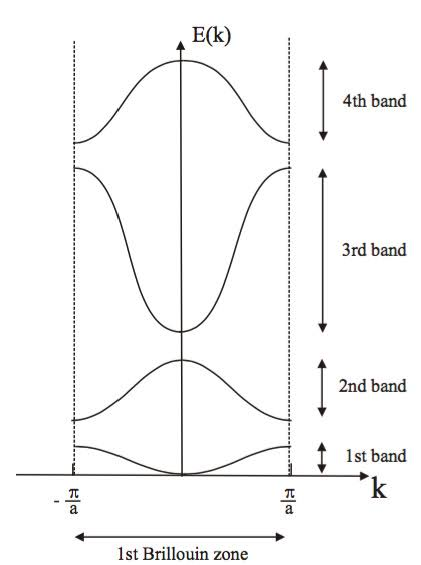
\includegraphics[scale=0.45]{./bands_in_first_brillouin_zone.jpg}
	\caption{Energy band inside the first Brillouin zone}
	\label{fig:firstbrillouinzone}
\end{figure}

\ex{1D example}{Let us use \begin{equation} V(x) = V_0\cos\frac{2\pi x}{a} \Rightarrow \tilde{V}(\pm\frac{2\pi}{a}) = \frac{V_0}{2}\end{equation} We can use this formula as it is written here because the delta functions are only defined in $\pm\frac{2\pi}{a}$ therefore we dont see the dirac functions, albeit they are there. Looking at the Bragg points:
\begin{equation} k_n = \frac{G_n}{2} = \frac{\pi}{2}n \end{equation} We can now draw the energy diagram.
\begin{center}
	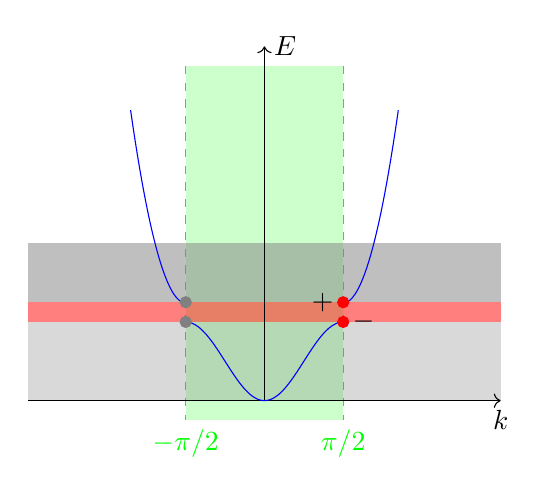
\begin{tikzpicture}
		\draw[dashed, green]	(1, 4.25) to (1, -0.25) node[below]{$\pi/2$};
		\draw[dashed, green]	(-1, 4.25) to (-1, -0.25) node[below]{$-\pi/2$};

		\fill[fill=green, opacity=0.2]	(1, 4.25) to (1, -0.25) to (-1, -0.25) to (-1, 4.25);
		\fill[fill=gray, opacity=0.3]	(-3, 1) to (-3, 0) to (3, 0) to (3, 1);
		\fill[fill=gray, opacity=0.5]	(-3, 1.25) to (-3, 2) to (3, 2) to (3, 1.25);
		\fill[fill=red, opacity=0.5]	(-3, 1) to (-3, 1.25) to (3, 1.25) to (3, 1);

		\draw[->, black] (0, 0) to (0, 4.5) node[right]{$E$};
		\draw[->, black] (-3, 0) to (3, 0) node[below]{$k$};

		\draw[domain=-1.7:-1, smooth, variable=\x, blue] plot ({\x}, {5*(\x + 1.2)*(\x + 0.8) + 1.44});
		\draw[domain=-1:1, smooth, variable=\x, blue] plot ({\x}, {sin((\x - 1/2)*180)/2+1/2});
		\draw[domain=1:1.7, smooth, variable=\x, blue] plot ({\x}, {5*(\x - 1.2)*(\x - 0.8) + 1.44});

		\filldraw[red] 	(1, 1) circle (2pt)
						(1, 1.25) circle (2pt);
		\filldraw[gray] (-1, 1.25) circle (2pt)
						(-1, 1) circle (2pt);

		\draw[black]	(1, 1) node[right]{$-$};
		\draw[black]	(1, 1.25) node[left]{$+$};
	\end{tikzpicture}
\end{center}
At the bragg points, we see a standing wave: $\psi_{\pm, k} \sim e^{i\pi x / a} \pm e^{-i\pi x/a}$, also shown in the figure in red. The bandgap is $V_0$ high.}

\chapter{Crystals} \label{ch:crystals}
\section{Crystal momentum}
Remember band diagrams derived in previous section \ref{sec:nearly_free_e_approx}. To introduce the crystal momentum, let's first look at
\begin{align}
	&\left\{
	\begin{array}{lr}
		\hat{H} = \frac{\hat{p}}{2m} = -\frac{\hbar^2}{2m}\nabla^2 \qquad\qquad \text{with: } \hat{\vec{p}} = -n\hbar\vec{\nabla}\\
		\hat{H}\psi_{\vec{k}}(\vec{r}) = E \psi_{\vec{k}}(\vec{r}) \\
		\psi_{\vec{k}} = \frac{1}{\sqrt{V}}e^{i\vec{k}\cdot\vec{r}}
	\end{array}\right\\
	&[\hat{H}, \hat{\vec{p}}] = 0\\
	\text{using de Brogli:}\qquad & \vec{p} = \hbar\vec{k} \label{eqn:brogli_relation}\\
	\text{we get:}\qquad &\hat{\vec{p}}\psi_{\vec{k}}(\vec{r}) = \hbar\vec{k}\psi_{\vec{k}}(\vec{r})
\end{align}
Bloch electrons: $\hat{H} = p^2/2m + V(\vec{r})$, with $\hat{\vec{p}} = -i\hbar\vec{\nabla}$.
Then now it is clear that these operators $[\hat{H}, \hat{\vec{p}}] \neq 0$
Then we can derive the following:
\begin{align}
	\hat{H}\psi_{n, \vec{k}}(\vec{r}) &= E_n(\vec{k})\psi_{n, \vec{k}}(\vec{r})\\
	\psi_{n, \vec{k}}(\vec{r}) &= u_{n, \vec{k}}(\vec{r})e^{i\vec{k}\cdot\vec{r}} \label{eqn:psi_bloch}\\
	\hat{\vec{p}}\psi_{n, \vec{k}}(\vec{r}) &= -i\hbar\vec{\nabla}\left[u_{n, \vec{k}}(\vec{r})e^{i\vec{k}\cdot\vec{r}}\right] \qquad \text{using: \ref{eqn:brogli_relation} and \ref{eqn:psi_bloch}}\\
\end{align}
How do we interpret the $\vec{k}$? Let's define crystal momentum as follows:
\begin{equation}
	\vec{P} = \hbar\vec{k}
\end{equation}
\nt{Don't confuse $\vec{P}$ with $\vec{p}$. For a Bloch electron we cannot say that $\vec{p} = \hbar\vec{k}$.}

Because real space is infinite, we need some boundary condiditions to confine our space.
\section{Boundary condition}
There are two possiblities to impose boundary conditions:
\begin{itemize}
	\setlength\itemsep{0pt}
	\item Dirichlet boundary conditions
	\item Born-von Kerman (periodic) boundary conditions
\end{itemize}
We will use periodic boundary conditions to show how energy bands are formed in an atomic crystal. The reason we use periodic boundary conditions is that this makes math easier, you do get the same result when using Dirichlet boundary conditions.
\ex{1D boundary condition}{
	For the function $\psi(x) = \psi(x + L)$, with $L$ the crystal length. 
	\begin{center}
		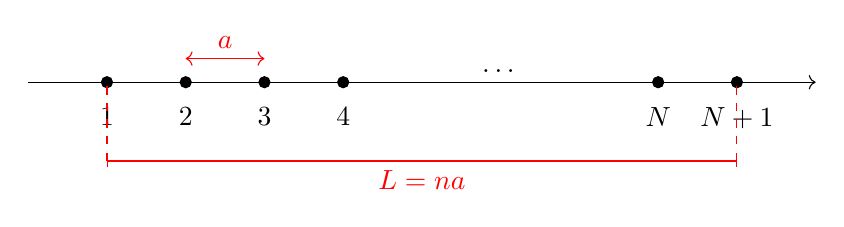
\begin{tikzpicture}
			\draw[->, black]	(0, 0) to (10, 0);

			\filldraw[black]	(1, 0) node[below=2mm]{$1$} circle (2pt)
								(2, 0) node[below=2mm]{$2$} circle (2pt)
								(3, 0) node[below=2mm]{$3$} circle (2pt)
								(4, 0) node[below=2mm]{$4$} circle (2pt)
								(8, 0) node[below=2mm]{$N$} circle (2pt)
								(9, 0) node[below=2mm]{$N+1$} circle (2pt);

			\draw[black]		(6, 0) node[above]{\dots};

			\draw[<->, red]		(2, 0.3) to node[above]{$a$} (3, 0.3);
			\draw[|-|, red]		(1, -1)	to node[below]{$L = na$} (9, -1);

			\draw[dashed, red]	(1, -1) to (1, 0)
								(9, -1) to (9, 0);
		\end{tikzpicture}
	\end{center}
	We can use some properties of the bloch functions, now we can deduce the following:
	\begin{align}
		\psi(x + L) &= e^{ikL}\psi(x) = \psi(x)\\
		&\Rightarrow kNa = 2\pi n \\
		&\Rightarrow k = \frac{2\pi}{L}n
	\end{align}
	We see that the continious $k$ value has become discrete, therefore we get the following figure. As we might expect, for a bigger lattice, we get a more continious spectrum (because $\Delta k$ becomes smaller).
	\begin{center}
		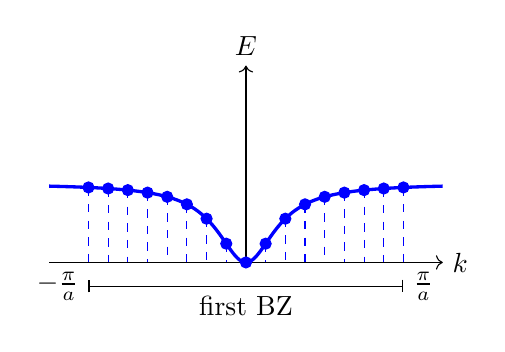
\begin{tikzpicture}[domain=-2.5:2.5]
			\draw[->] (-2.5,0) -- (2.5,0) node[right] {$k$};
			\draw[->] (0,0) -- (0,2.5) node[above] {$E$};

			\draw[blue, very thick] plot[samples=200] (\x, {1 - 1/(1 + 5*\x*\x)});

			\foreach \x in {-8,...,8} {
				\filldraw[blue]	({\x / 4}, {1 - 1/(1 + 5*\x*\x / 16)}) circle (2pt);
				\draw[dashed, blue]	({\x / 4}, {1 - 1/(1 + 5*\x*\x / 16)}) to ({\x / 4}, 0);
			}

			\draw	(-2, -0.3)	node[left]{$-\frac{\pi}{a}$};
			\draw	(2, -0.3)	node[right]{$\frac{\pi}{a}$};

			\draw[|-|]	(-2, -0.3) to node[below]{first BZ} (2, -0.3);
		\end{tikzpicture}
	\end{center}
	How many lattice points do we have in our first BZ?
	\begin{equation}
		\frac{\frac{2\pi}{a}}{\Delta k} = \frac{\frac{2\pi}{a}}{\frac{2\pi}{Na}} = N = \text{number of unit cells that build the crystal}
	\end{equation}
}
Can we come to the same conclusion in 3D?
\ex{3D boundary condition}{
	The full crystal is defined by $L_1$, $L_2$, $L_3$. For these values, we can say that:
	\begin{align}
		\left\{
		\begin{array}{lr}
		\vec{L_1} = N_1\vec{a}_1\\
		\vec{L_2} = N_2\vec{a}_2\\
		\vec{L_3} = N_3\vec{a}_3
		\end{array}
		\right
	\end{align}
	We can do the same as we did in the 1D example:
	\begin{align}
		\psi(\vec{r} + \vec{L}_j) &= \psi(\vec{r})\\
		&= \psi(\vec{r} + N_j\vec{a}_j)\\
		\text{Using Bloch}\qquad &\Rightarrow \psi(\vec{r}) = e^{i\vec{k}\cdotN_j\vec{a}_j}\psi(\vec{r})\\
		&\Rightarrow \vec{k} = 2\pi n \cdot (N_j \vec{a}_j)^{-1} \text{with } n \in \bbZ\\
		&\Rightarrow \vec{k} = \frac{n_1}{N_1}\vec{b}_1 + \frac{n_2}{N_2}\vec{b}_2 + \frac{n_3}{N_3}\vec{b}_3
	\end{align}

	$\vec{b}_i$ are primitive reciprocal lattice vectors.

	Now we look at the elemental volume of the unit cell:
	\begin{align}
		\Delta \vec{k} = \Delta k^3 &= \frac{\vec{b}_1}{N_1}\cdot\left(\frac{\vec{b}_2}{N_2} \cross \frac{\vec{b}_3}{N_3}\right)\\
		&= \frac{1}{N}\vec{b}_1\cdot\left(\vec{b}_2 \cross \vec{b}_3\right)
	\end{align}
	Where N is the number of unit cells that build the crystal.
}
We do get the same results, and this has some consequences when we look at the atomic picture of energy bands and how boundary conditions affect them.
\begin{enumerate}
	\setlength\itemsep{0pt}
	\item Even number of electrons in a full shell per unit cell. We get $2N =$ amount of electrons. This gives a semiconductor.
	\item Odd number of electrons in apartially filled shell per unit cell. Because there are still states free in the valence band, gives this a metal.
\end{enumerate}
\nt{This does not mean that a $2N$ amount of electrons gives a semiconductor. Band overlap can still give a metal!}
We now link this concept to real atoms.

\section{Energy bands for the atomic picture} \label{sec:atomic_picture}
Say, we have $N$ atoms. Then, for each atom we have the states in figure \ref{fig:state_one_atom}. Now suppose we have them far apart and bring them closer, then we get figure \ref{fig:bands_crystal_fictiveatoms}. For a semiconductor, we see a bandgap $E_g$ at $d = a$, this is highlighted in red.
\begin{figure}[h]
	\centering
	\begin{tikzpicture}
		\draw[-, black, very thick]	(0, 0) to (3, 0) node[right]{1s}
									(0, 2) to (3, 2) node[right]{2s};

		\draw[->, black]	(-0.5, -0.5) to (-0.5, 2.5) node[right]{$E$};
	\end{tikzpicture}
	\caption{The energy state for a fictive single atom}
	\label{fig:state_one_atom}
\end{figure}
\begin{figure}[h]
	\centering
	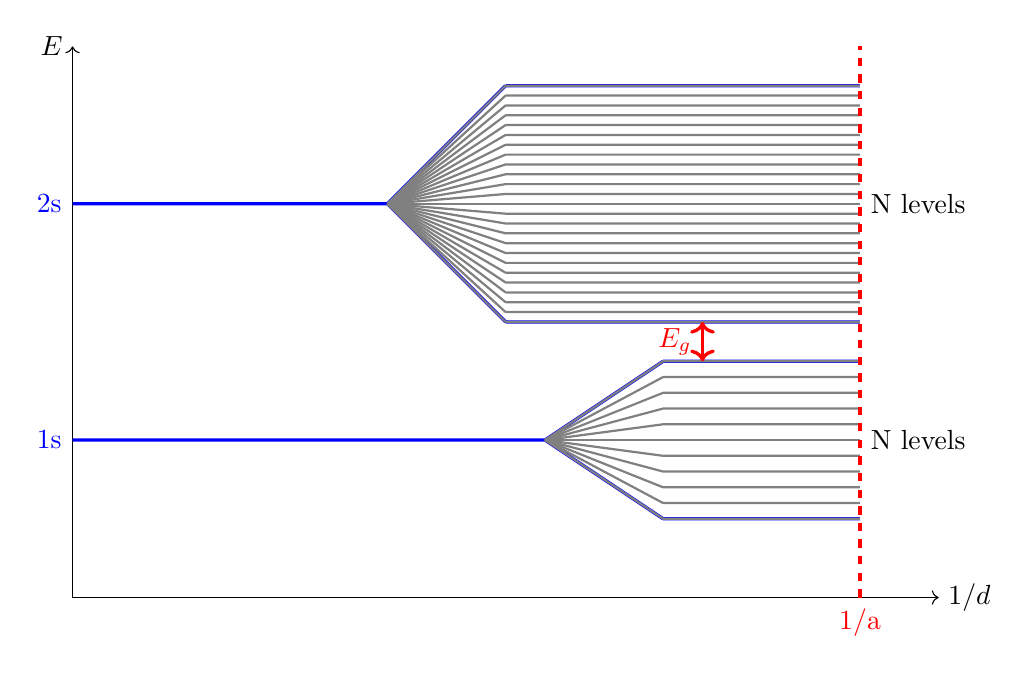
\begin{tikzpicture}
		\draw[->, black]	(0, 0) to (0, 7) node[left]{$E$};
		\draw[->, black]	(0, 0) to (11, 0) node[right]{$1/d$};

		\draw[-, blue, very thick]		(0, 2) node[left]{1s} to (6, 2)
							(6, 2) to (7.5, 3)
							(6, 2) to (7.5, 1)
							(7.5, 3) to (10, 3)
							(7.5, 1) to (10, 1);

		\draw[-, blue, very thick]		(0, 5) node[left]{2s} to (4, 5)
							(4, 5) to (5.5, 6.5)
							(4, 5) to (5.5, 3.5)
							(5.5, 6.5) to (10, 6.5)
							(5.5, 3.5) to (10, 3.5);

		\foreach \y in {28, ..., 52} {
			\draw[-, gray, thick]	(5.5, {\y/8}) to (10, {\y/8})
									(4, 5) to (5.5, {\y/8});
		}

		\foreach \y in {5, ..., 15} {
			\draw[-, gray, thick]	(7.5, {\y/5}) to (10, {\y/5})
									(6, 2) to (7.5, {\y/5});
		}

		\draw[red, very thick]	(10, 0) node[below]{1/a};
		\draw[dashed, red, very thick]	(10, 0) to (10, 7);

		\draw[black, very thick]	(10, 5) node[right]{N levels};
		\draw[black, very thick]	(10, 2) node[right]{N levels};

		\draw[<->, red, very thick]	(8, 3) to node[left]{$E_g$} (8, 3.5);
	\end{tikzpicture}
	\caption{Energy band diagram for fictive crystal of N atoms}
	\label{fig:bands_crystal_fictiveatoms}
\end{figure}
This just shows how the bands are for the atoms, nothig can be said about momentum, \dots. What we notice from the picture, too is:
\begin{itemize}
	 \setlength\itemsep{0pt}
	\item 2s orbital starts to split sooner, because 2s oribitals overlap more as they are furhter away from the nucleus.
	\item We see a smaller band splitting at 1s.
\end{itemize}
We will now look at some other atoms.
\newpage
\ex{Lithium (Li)}{
	For 1 Li atom we have what can be seen in following figure:
	\begin{center}
		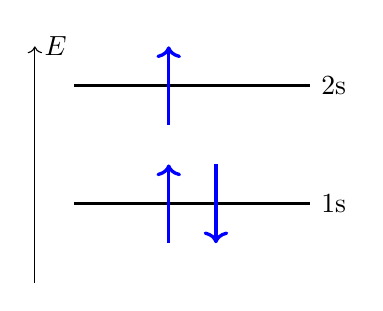
\begin{tikzpicture}
			\draw[-, black, very thick]	(0, 0.5) to (3, 0.5) node[right]{1s}
										(0, 2) to (3, 2) node[right]{2s};

			\draw[->, blue, very thick]	(1.2, 0) to (1.2, 1);
			\draw[->, blue, very thick]	(1.8, 1) to (1.8, 0);
			\draw[->, blue, very thick]	(1.2, 1.5) to (1.2, 2.5);

			\draw[->, black]	(-0.5, -0.5) to (-0.5, 2.5) node[right]{$E$};
		\end{tikzpicture}
	\end{center}

	For $Li_2$ we get:
	\begin{center}
		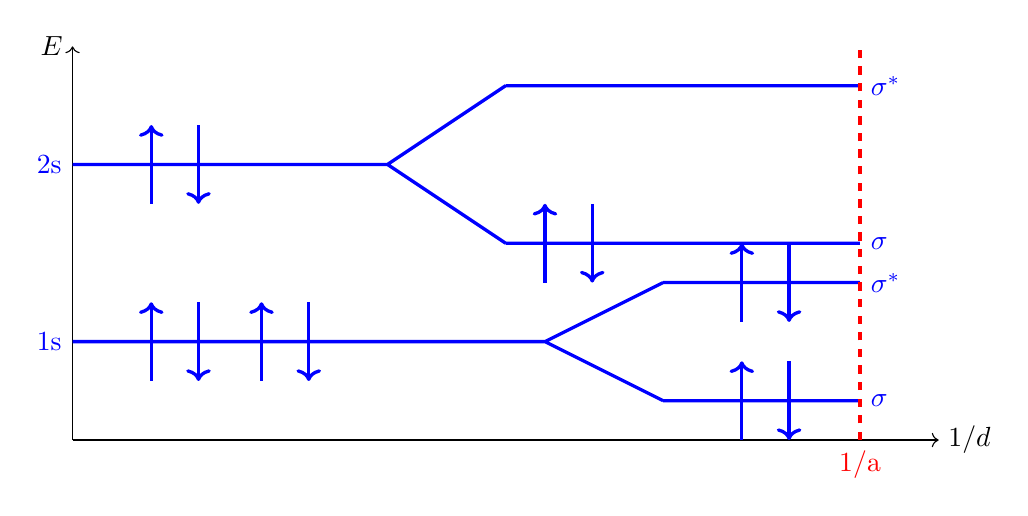
\begin{tikzpicture}
			\draw[->, black]	(0, 0) to (0, 5) node[left]{$E$};
			\draw[->, black]	(0, 0) to (11, 0) node[right]{$1/d$};

			\draw[-, blue, very thick]		(0, 1.25) node[left]{1s} to (6, 1.25)
								(6, 1.25) to (7.5, 2)
								(6, 1.25) to (7.5, 0.5)
								(7.5, 2) to (10, 2) node[right]{$\sigma^{*}$}
								(7.5, 0.5) to (10, 0.5) node[right]{$\sigma$};

			\draw[-, blue, very thick]		(0, 3.5) node[left]{2s} to (4, 3.5)
								(4, 3.5) to (5.5, 4.5)
								(4, 3.5) to (5.5, 2.5)
								(5.5, 4.5) to (10, 4.5) node[right]{$\sigma^{*}$}
								(5.5, 2.5) to (10, 2.5) node[right]{$\sigma$};

			\draw[red, very thick]	(10, 0) node[below]{1/a};
			\draw[dashed, red, very thick]	(10, 0) to (10, 5);

			\draw[->, blue, very thick]	(1, 0.75) to (1, 1.75);
			\draw[->, blue, very thick]	(1.6, 1.75) to (1.6, 0.75);
			\draw[->, blue, very thick]	(2.4, 0.75) to (2.4, 1.75);
			\draw[->, blue, very thick]	(3, 1.75) to (3, 0.75);
			\draw[->, blue, very thick]	(1, 3) to (1, 4);
			\draw[->, blue, very thick]	(1.6, 4) to (1.6, 3);
			\draw[->, blue, very thick]	(8.5, 0) to (8.5, 1);
			\draw[->, blue, very thick]	(9.1, 1) to (9.1, 0);
			\draw[->, blue, very thick]	(8.5, 1.5) to (8.5, 2.5);
			\draw[->, blue, very thick]	(9.1, 2.5) to (9.1, 1.5);
			\draw[->, blue, very thick]	(6, 2) to (6, 3);
			\draw[->, blue, very thick]	(6.6, 3) to (6.6, 2);
		\end{tikzpicture}
	\end{center}

	For a crystal $Li_N$ we get:
	\begin{center}
		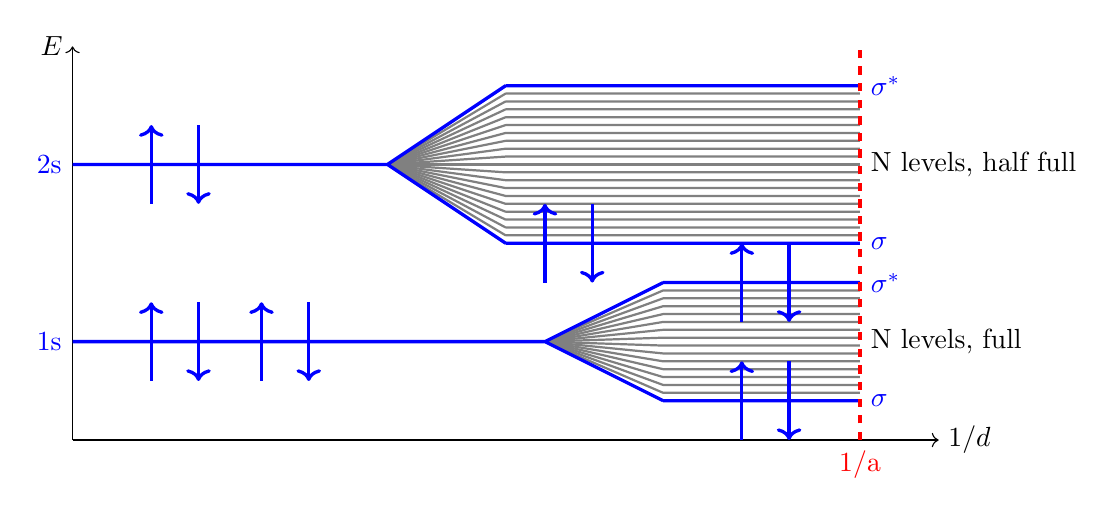
\begin{tikzpicture}
			\draw[->, black]	(0, 0) to (0, 5) node[left]{$E$};
			\draw[->, black]	(0, 0) to (11, 0) node[right]{$1/d$};

			\foreach \y in {5, ..., 20} {
				\draw[-, gray, thick]	(7.5, {\y/10}) to (10, {\y/10})
										(6, 1.25) to (7.5, {\y/10});
			}

			\draw[-, blue, very thick]		(0, 1.25) node[left]{1s} to (6, 1.25)
								(6, 1.25) to (7.5, 2)
								(6, 1.25) to (7.5, 0.5)
								(7.5, 2) to (10, 2) node[right]{$\sigma^{*}$}
								(7.5, 0.5) to (10, 0.5) node[right]{$\sigma$};

			\foreach \y in {25, ..., 45} {
				\draw[-, gray, thick]	(5.5, {\y/10}) to (10, {\y/10})
										(4, 3.5) to (5.5, {\y/10});
			}

			\draw[-, blue, very thick]		(0, 3.5) node[left]{2s} to (4, 3.5)
								(4, 3.5) to (5.5, 4.5)
								(4, 3.5) to (5.5, 2.5)
								(5.5, 4.5) to (10, 4.5) node[right]{$\sigma^{*}$}
								(5.5, 2.5) to (10, 2.5) node[right]{$\sigma$};

			\draw[red, very thick]	(10, 0) node[below]{1/a};
			\draw[dashed, red, very thick]	(10, 0) to (10, 5);

			\draw[->, blue, very thick]	(1, 0.75) to (1, 1.75);
			\draw[->, blue, very thick]	(1.6, 1.75) to (1.6, 0.75);
			\draw[->, blue, very thick]	(2.4, 0.75) to (2.4, 1.75);
			\draw[->, blue, very thick]	(3, 1.75) to (3, 0.75);
			\draw[->, blue, very thick]	(1, 3) to (1, 4);
			\draw[->, blue, very thick]	(1.6, 4) to (1.6, 3);
			\draw[->, blue, very thick]	(8.5, 0) to (8.5, 1);
			\draw[->, blue, very thick]	(9.1, 1) to (9.1, 0);
			\draw[->, blue, very thick]	(8.5, 1.5) to (8.5, 2.5);
			\draw[->, blue, very thick]	(9.1, 2.5) to (9.1, 1.5);
			\draw[->, blue, very thick]	(6, 2) to (6, 3);
			\draw[->, blue, very thick]	(6.6, 3) to (6.6, 2);

			\draw[black, very thick]	(10, 3.5) node[right]{N levels, half full};
			\draw[black, very thick]	(10, 1.25) node[right]{N levels, full};
		\end{tikzpicture}
	\end{center}
}
\ex{Silicium (Si)}{
	Si has following configuration: $1s^2\,2s^2\,2p^6\,3s^2\,3p^2$. This translates in the following band structure:
	\begin{center}
		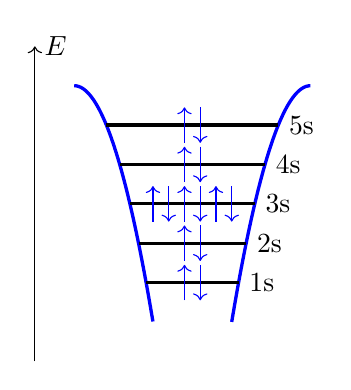
\begin{tikzpicture}
			\draw[blue, very thick] plot[samples=200, domain=0:1] (\x, {-3*\x*\x + 3});
			\draw[blue, very thick] plot[samples=200, domain=2:3] (\x, {-3*(\x - 3)*(\x - 3) + 3});

			\foreach \y in {1, ..., 5} {
				\draw[-, black, very thick]	({ ((\y/2 - 3)/-3)^(1/2) }, \y/2) to ( {-((\y/2 - 3)/-3)^(1/2) + 3}, \y/2) node[right]{\text{\y}s};

				\draw[->, blue]	(1.4, \y/2 - 0.225) to (1.4, {\y/2 + 0.225});
				\draw[->, blue]	(1.6, {\y/2 + 0.225}) to (1.6, \y/2 - 0.225);
			}

			\draw[->, blue]	({1.4 - 0.4}, {3/2 - 0.225}) to ({1.4 - 0.4}, {3/2 + 0.225});
			\draw[->, blue]	({1.6 - 0.4}, {3/2 + 0.225}) to ({1.6 - 0.4}, {3/2 - 0.225});

			\draw[->, blue]	({1.4 + 0.4}, {3/2 - 0.225}) to ({1.4 + 0.4}, {3/2 + 0.225});
			\draw[->, blue]	({1.6 + 0.4}, {3/2 + 0.225}) to ({1.6 + 0.4}, {3/2 - 0.225});

			\draw[->, black]	(-0.5, -0.5) to (-0.5, 3.5) node[right]{$E$};
		\end{tikzpicture}
	\end{center}
	For a Si crystal we have $N$ unit cells. Si cyrstals have a diamond structure with 2 atoms per unit cell. The according band diagram is:
	\begin{center}
		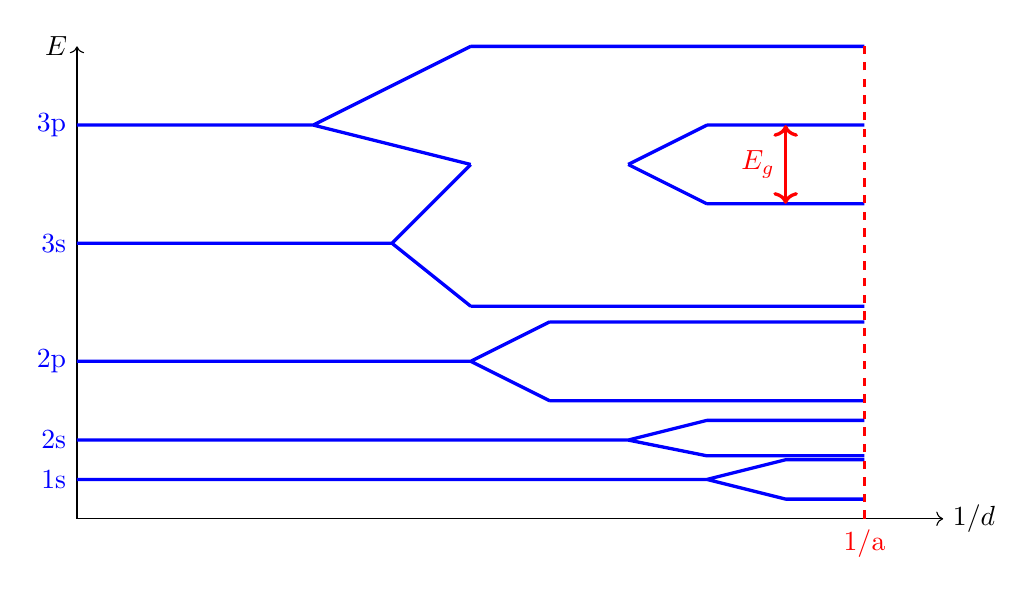
\begin{tikzpicture}
			\draw[->, black]	(0, 0) to (0, 6) node[left]{$E$};
			\draw[->, black]	(0, 0) to (11, 0) node[right]{$1/d$};

			\draw[-, blue, very thick]		(0, 0.5) node[left]{1s} to (8, 0.5)
											(8, 0.5) to (9, 0.25)
											(8, 0.5) to (9, 0.75)
											(9, 0.25) to (10, 0.25)
											(9, 0.75) to (10, 0.75);

			\draw[-, blue, very thick]		(0, 1) node[left]{2s} to (7, 1)
											(7, 1) to (8, 1.25)
											(7, 1) to (8, 0.8)
											(8, 1.25) to (10, 1.25)
											(8, 0.8) to (10, 0.8);

			\draw[-, blue, very thick]		(0, 2) node[left]{2p} to (5, 2)
											(5, 2) to (6, 2.5)
											(5, 2) to (6, 1.5)
											(6, 2.5) to (10, 2.5)
											(6, 1.5) to (10, 1.5);

			\draw[-, blue, very thick]		(0, 3.5) node[left]{3s} to (4, 3.5)
											(4, 3.5) to (5, 4.5)
											(4, 3.5) to (5, 2.7)
											(5, 2.7) to (10, 2.7)
											(7, 4.5) to (8, 4)
											(8, 4) to (10, 4);

			\draw[-, blue, very thick]		(0, 5) node[left]{3p} to (3, 5)
											(3, 5) to (5, 6)
											(3, 5) to (5, 4.5)
											(5, 6) to (10, 6)
											(7, 4.5) to (8, 5)
											(8, 5) to (10, 5);

			\draw[red, very thick]	(10, 0) node[below]{1/a};
			\draw[dashed, red, very thick]	(10, 0) to (10, 6);

			\draw[<->, red, very thick]	(9, 4) to node[left]{$E_g$} (9, 5);
		\end{tikzpicture}
	\end{center}
	If we now consider that each each unit cell has 2 atoms in a silicon lattice, we get the following states for the energy diagram (simplified):
	\begin{center}
		\begin{tikzpicture}
			\draw[->, black]	(0, 0) to (0, 6) node[left]{$E$};
			\draw[->, black]	(0, 0) to (11, 0) node[right]{$1/d$};

			\foreach \y in {2.5, ..., 7.5} {
				\draw[-, gray, thick]	(9, {\y/10}) to (10, {\y/10})
										(8, 0.5) to (9, {\y/10});
			}

			\foreach \y in {8, ..., 12.5} {
				\draw[-, gray, thick]	(8, {\y/10}) to (10, {\y/10})
										(7, 1) to (8, {\y/10});
			}

			\foreach \y in {15, ..., 25} {
				\draw[-, gray, thick]	(6, {\y/10}) to (10, {\y/10})
										(5, 2) to (6, {\y/10});
			}

			\foreach \y in {27, ..., 45} {
				\draw[-, gray, thick]	(5, {\y/10}) to (7, {\y/10})
										(4, 3.5) to (5, {\y/10})
										(7, {\y/10}) to (8, {\y/15 + 0.9})
										(8, {\y/15 + 0.9}) to (10, {\y/15 + 0.9});
			}

			\foreach \y in {45, ..., 60} {
				\draw[-, gray, thick]	(5, {\y/10}) to (7, {\y/10})
										(3, 5) to (5, {\y/10})
										(7, {\y/10}) to (8, {\y/16 + 2.2})
										(8, {\y/16 + 2.2}) to (10, {\y/16 + 2.2});
			}

			\draw[-, blue, very thick]		(0, 0.5) node[left]{1s} to (8, 0.5)
											(8, 0.5) to (9, 0.25)
											(8, 0.5) to (9, 0.75)
											(9, 0.25) to (10, 0.25)
											(9, 0.75) to (10, 0.75);

			\draw[-, blue, very thick]		(0, 1) node[left]{2s} to (7, 1)
											(7, 1) to (8, 1.25)
											(7, 1) to (8, 0.8)
											(8, 1.25) to (10, 1.25)
											(8, 0.8) to (10, 0.8);

			\draw[-, blue, very thick]		(0, 2) node[left]{2p} to (5, 2)
											(5, 2) to (6, 2.5)
											(5, 2) to (6, 1.5)
											(6, 2.5) to (10, 2.5)
											(6, 1.5) to (10, 1.5);

			\draw[-, blue, very thick]		(0, 3.5) node[left]{3s} to (4, 3.5)
											(4, 3.5) to (5, 4.5)
											(4, 3.5) to (5, 2.7)
											(5, 2.7) to (10, 2.7)
											(7, 4.5) to (8, 4)
											(8, 4) to (10, 4);

			\draw[-, blue, very thick]		(0, 5) node[left]{3p} to (3, 5)
											(3, 5) to (5, 6)
											(3, 5) to (5, 4.5)
											(5, 6) to (10, 6)
											(7, 4.5) to (8, 5)
											(8, 5) to (10, 5);

			\draw[red, very thick]	(10, 0) node[below]{1/a};
			\draw[dashed, red, very thick]	(10, 0) to (10, 6);

			\draw[<->, red, very thick]	(9, 4) to node[left]{$E_g$} (9, 5);

			\draw[black]	(2, 3.5) node[above]{$4N$ electrons} node[below]{$4N$ states possible};
			\draw[black]	(1.5, 5) node[above]{$4N$ electrons} node[below]{$12N$ states possible};

			\draw[-, magenta, thick]	(3.2, 6.1) node[above]{Partially filled band ($6N$)} to (4.9, 6.1) to (4.9, 4.5) to (3.2, 4.5) to (3.2, 6.1);
			\draw[-, orange, thick]	(5.1, 6.1) to (6.9, 6.1) to (6.9, 2.6) to (5.1, 2.6) node[left]{Partially filled band ($8N$)} to (5.1, 6.1);
			\draw[black]	(10, 5.5) node[right]{$8N$ states; empty}
		\end{tikzpicture}
	\end{center}
	All possible states for the valence bands can be found on the picture.
}

\subsection{Higer dimension energy band diagrams}
We can represent these band configurations in k-space, too, but these plots can get complicated. Luckily, there is a solution for that. This concept is illustrated with picture \ref{fig:banddiagram_silicon}. We will travel along the following path: $\Gamma - K - M - \Gamma$. This gives a plot that has enough information about the crystal. Thus plotting $E(\vec{k})$ along the high symmetry points, in the first BZ, is adequate for determining the behaviour of the cyrstals in higher dimensions. The lines we follow are called \textbf{Bragg-lines}. The only thing we want to get to know is what the maximum/minimum of the valence/conduction band are. This is acheived with the Bragg-lines.
\begin{figure}
	\centering
	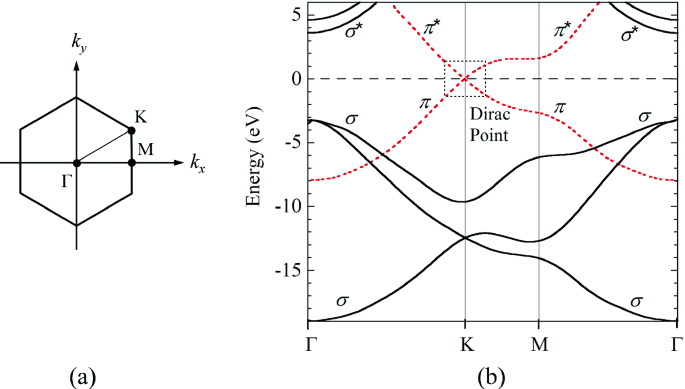
\includegraphics[scale=0.5]{./banddiagram_silicon.png}
	\caption{2D banddiagram for silicon}
	\label{fig:banddiagram_silicon}
\end{figure}

\section{Implications of the periodic boundary condition}
\dfn{Amount of allowed $\vec{k}$-states, N}{
	The amount of allowed $\vec{k}$-states, N, is given by the amount of unit cells that build the crystal. This implicates that in each energy band $E_n(\vec{k})$, where $\vec{k} \in$ first BZ, there are N allowed $\vec{k}$-states.
}

There are serveral cases we can study, we will go over them.

\subsection{Case 1 - N is odd}
Take the amount of valence electrons in each unit cell is odd. If we consider the first BZ we get the energy band structure that is given in figure \ref{fig:N_odd_band_struct}. For each $\vec{k}$-state, we can have two electrons: spin up and spin down. Ìn this picture, the circles decpict a hole. Furthermore, the temperature in this figure is $0K$, all electrons are in their base state.\par
Now, the fact that we have an odd number of electrons, we need to have partially filled bands. In this case we have metallic crystals.
\begin{figure}[h]
	\centering
	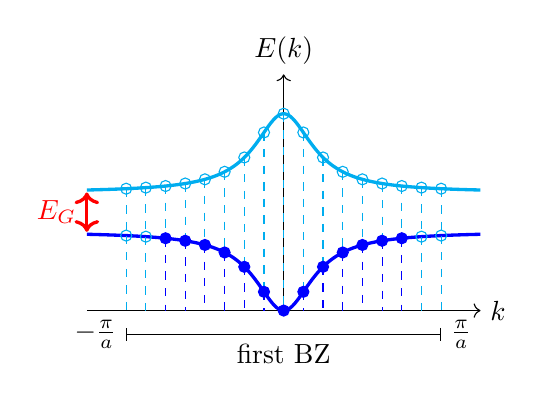
\begin{tikzpicture}[domain=-2.5:2.5]
		\draw[->] (-2.5,0) -- (2.5,0) node[right] {$k$};
		\draw[->] (0,0) -- (0, 3) node[above] {$E(k)$};

		\draw[blue, very thick] plot[samples=200] (\x, {1 - 1/(1 + 5*\x*\x)});
		\draw[cyan, very thick] plot[samples=200] (\x, {1.5 + 1/(1 + 5*\x*\x)});

		\draw[<->, red, very thick]	(-2.5, 1) to node[left]{$E_G$} (-2.5, 1.5);

		\foreach \x in {-8,...,8} {
			\draw[cyan]	({\x / 4}, {1.5 + 1/(1 + 5*\x*\x / 16)}) circle (2pt);
			\draw[dashed, cyan]	({\x / 4}, {1.5 + 1/(1 + 5*\x*\x / 16)}) to ({\x / 4}, {1 - 1/(1 + 5*\x*\x / 16)});
		}

		\foreach \x in {-8,...,8} {
			\ifnum \x < -6 {
				\draw[cyan]	({\x / 4}, {1 - 1/(1 + 5*\x*\x / 16)}) circle (2pt);
				\draw[dashed, cyan]	({\x / 4}, {1 - 1/(1 + 5*\x*\x / 16)}) to ({\x / 4}, 0);
			}
			\else {
				\ifnum \x > 6 {
					\draw[cyan]	({\x / 4}, {1 - 1/(1 + 5*\x*\x / 16)}) circle (2pt);
					\draw[dashed, cyan]	({\x / 4}, {1 - 1/(1 + 5*\x*\x / 16)}) to ({\x / 4}, 0);
				}
				\else {
					\filldraw[blue]	({\x / 4}, {1 - 1/(1 + 5*\x*\x / 16)}) circle (2pt);
					\draw[dashed, blue]	({\x / 4}, {1 - 1/(1 + 5*\x*\x / 16)}) to ({\x / 4}, 0);
				} \fi
			} \fi
		}

		\draw	(-2, -0.3)	node[left]{$-\frac{\pi}{a}$};
		\draw	(2, -0.3)	node[right]{$\frac{\pi}{a}$};

		\draw[|-|]	(-2, -0.3) to node[below]{first BZ} (2, -0.3);
	\end{tikzpicture}
	\caption{Band structure with odd number of electrons}
	\label{fig:N_odd_band_struct}
\end{figure}
\subsection{Case 2 - N is even}
The amount of electrons in each unit cell is even. Again, we consider the first BZ. We get figure \ref{fig:N_even_band_struct}. Now we speak about a semiconductor (or an insulator if $E_G$ is large).
\begin{figure}[h]
	\centering
	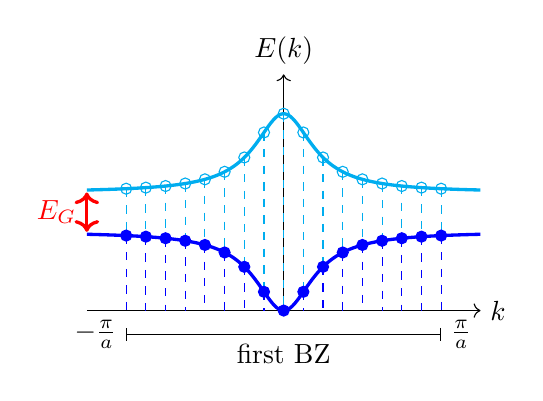
\begin{tikzpicture}[domain=-2.5:2.5]
		\draw[->] (-2.5,0) -- (2.5,0) node[right] {$k$};
		\draw[->] (0,0) -- (0, 3) node[above] {$E(k)$};

		\draw[blue, very thick] plot[samples=200] (\x, {1 - 1/(1 + 5*\x*\x)});
		\draw[cyan, very thick] plot[samples=200] (\x, {1.5 + 1/(1 + 5*\x*\x)});

		\draw[<->, red, very thick]	(-2.5, 1) to node[left]{$E_G$} (-2.5, 1.5);

		\foreach \x in {-8,...,8} {
			\draw[cyan]	({\x / 4}, {1.5 + 1/(1 + 5*\x*\x / 16)}) circle (2pt);
			\draw[dashed, cyan]	({\x / 4}, {1.5 + 1/(1 + 5*\x*\x / 16)}) to ({\x / 4}, {1 - 1/(1 + 5*\x*\x / 16)});
		}

		\foreach \x in {-8,...,8} {
			\filldraw[blue]	({\x / 4}, {1 - 1/(1 + 5*\x*\x / 16)}) circle (2pt);
			\draw[dashed, blue]	({\x / 4}, {1 - 1/(1 + 5*\x*\x / 16)}) to ({\x / 4}, 0);
		}

		\draw	(-2, -0.3)	node[left]{$-\frac{\pi}{a}$};
		\draw	(2, -0.3)	node[right]{$\frac{\pi}{a}$};

		\draw[|-|]	(-2, -0.3) to node[below]{first BZ} (2, -0.3);
	\end{tikzpicture}
	\caption{Band structure with odd number of electrons}
	\label{fig:N_even_band_struct}
\end{figure}
\subsection{Case 3 - N is even + band overlap}
The amount of electrons in the crystal is even and we have a band overlap. We now get a figure as figure \ref{fig:N_even_band_struct_w_overlap}. As you might guess, we get a metal again. Because now the electrons can move in their energyband when an electric field is applied.
\begin{figure}[h]
	\centering
	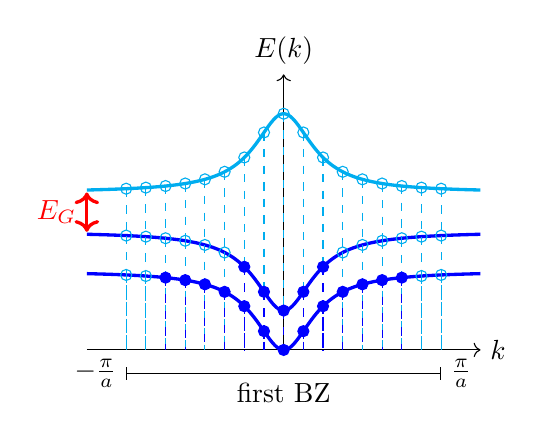
\begin{tikzpicture}[domain=-2.5:2.5]
		\draw[->] (-2.5,0) -- (2.5,0) node[right] {$k$};
		\draw[->] (0,0) -- (0, 3.5) node[above] {$E(k)$};

		\draw[blue, very thick] plot[samples=200] (\x, {1 - 1/(1 + 5*\x*\x)});
		\draw[blue, very thick] plot[samples=200] (\x, {1.5 - 1/(1 + 5*\x*\x)});
		\draw[cyan, very thick] plot[samples=200] (\x, {2 + 1/(1 + 5*\x*\x)});

		\draw[<->, red, very thick]	(-2.5, 1.5) to node[left]{$E_G$} (-2.5, 2);

		\foreach \x in {-8,...,8} {
			\draw[cyan]	({\x / 4}, {2 + 1/(1 + 5*\x*\x / 16)}) circle (2pt);
			\draw[dashed, cyan]	({\x / 4}, {2 + 1/(1 + 5*\x*\x / 16)}) to ({\x / 4}, {1.5 - 1/(1 + 5*\x*\x / 16)});
		}

		\foreach \x in {-8,...,8} {
			\ifnum \x < -2 {
				\draw[cyan]	({\x / 4}, {1.5 - 1/(1 + 5*\x*\x / 16)}) circle (2pt);
				\draw[dashed, cyan]	({\x / 4}, {1.5 - 1/(1 + 5*\x*\x / 16)}) to ({\x / 4}, 0);
			}
			\else {
				\ifnum \x > 2 {
					\draw[cyan]	({\x / 4}, {1.5 - 1/(1 + 5*\x*\x / 16)}) circle (2pt);
					\draw[dashed, cyan]	({\x / 4}, {1.5 - 1/(1 + 5*\x*\x / 16)}) to ({\x / 4}, 0);
				}
				\else {
					\filldraw[blue]	({\x / 4}, {1.5 - 1/(1 + 5*\x*\x / 16)}) circle (2pt);
					\draw[dashed, blue]	({\x / 4}, {1.5 - 1/(1 + 5*\x*\x / 16)}) to ({\x / 4}, 0);
				} \fi
			} \fi
		}

		\foreach \x in {-8,...,8} {
			\ifnum \x < -6 {
				\draw[cyan]	({\x / 4}, {1 - 1/(1 + 5*\x*\x / 16)}) circle (2pt);
				\draw[dashed, cyan]	({\x / 4}, {1 - 1/(1 + 5*\x*\x / 16)}) to ({\x / 4}, 0);
			}
			\else {
				\ifnum \x > 6 {
					\draw[cyan]	({\x / 4}, {1 - 1/(1 + 5*\x*\x / 16)}) circle (2pt);
					\draw[dashed, cyan]	({\x / 4}, {1 - 1/(1 + 5*\x*\x / 16)}) to ({\x / 4}, 0);
				}
				\else {
					\filldraw[blue]	({\x / 4}, {1 - 1/(1 + 5*\x*\x / 16)}) circle (2pt);
					\draw[dashed, blue]	({\x / 4}, {1 - 1/(1 + 5*\x*\x / 16)}) to ({\x / 4}, 0);
				} \fi
			} \fi
		}

		\draw	(-2, -0.3)	node[left]{$-\frac{\pi}{a}$};
		\draw	(2, -0.3)	node[right]{$\frac{\pi}{a}$};

		\draw[|-|]	(-2, -0.3) to node[below]{first BZ} (2, -0.3);
	\end{tikzpicture}
	\caption{Band structure with odd number of electrons}
	\label{fig:N_even_band_struct_w_overlap}
\end{figure}

\section{Calculating the band structre \& solving for the bandstructure}
How do we get the bands? By just calculating the Schödinger equations, of course. Remember we did this for a free electron in section \ref{sec:nearly_free_e_approx}. There, we solved the equation:
\begin{equation}
	\left[-\frac{\hbar^2}{2m}\nabla^2 + V(\vec{r})\right]\psi_{n, \vec{k}}(\vec{r}) = E_n(\vec{k})\psi_{n, \vec{k}}(\vec{r})
\end{equation}
There are also other methods, i.e., the Tight Binding approach. This method is more representative for the band diagrams drawn in section \ref{sec:atomic_picture}. In the Tight Binding approximation, one writes the atomic and electronic part seperatly, which leads to solving the above Schrödinger equation in terms of atomic orbitals. The atomic orbitals are the ones we have drawn in section \ref{sec:atomic_picture}.\par
The prediction of the atomic orbitals, as given in section \ref{sec:atomic_picture}, cannot be predicted with the nearly free electron approximation. In this approximation, it seems as if all orbitals are s-orbitals. Where both Tight Binding and Nearly Free electron approximation do predict right is the placement of the bandgap, which is at the Bragg-points.


\end{document}
